 	 \documentclass{beamer} %  [handout]  -> streicht die pause raus


\usepackage{dsfont} %Double stroke, e.g. for indicator function

%%%BASICS
\usepackage[utf8]{inputenc}
\usepackage{csquotes}
\usepackage{amssymb}

%%%START THEME SETTINGS

% IFO BLAU!!!
\setbeamercolor{structure}{fg=beamer@ifoblue}
\definecolor{beamer@ifoblue}{RGB}{12,50,82}
%\definecolor{ifoblue}{RGB}{12,50,82}

\usetheme{Hannover}
\usecolortheme{dolphin}
\usefonttheme{professionalfonts}




%%%END THEME SETTINGS

\usepackage[compatibility=false]{caption}
\usepackage{subcaption}
\usepackage{graphicx} 
%PATH MAC
%\graphicspath{{/Users/marcfabel/Dropbox/Uni/Tinbergen/MPhil/STATA/GRAPHS/}}

%F:\_MPhil\STATA\graphs
%PATH Windows
%\graphicspath{{F:/_MPhil/STATA/graphs/}}
%\graphicspath{{C:/Users/fabel/Dropbox/Uni/Tinbergen/MPhil/STATA/GRAPHS/}}

\usepackage{afterpage}
 \usepackage{hyperref}
\usepackage{booktabs}
\usepackage[labelfont=bf,labelsep = period, singlelinecheck=off,justification=raggedright]{caption}%both together help to have subfigures, other specifications which are nice: labelformat = parens -> number in paranthesis
\usepackage[singlelinecheck=on]{subcaption}


\setbeamertemplate{items}[circle]
\usepackage{tikz}
\newcommand\mynum[1]{%
  \usebeamercolor{enumerate item}%
  \tikzset{beameritem/.style={circle,inner sep=0,minimum size=2ex,text=enumerate item.bg,fill=enumerate item.fg,font=\footnotesize}}%
  \tikz[baseline=(n.base)]\node(n)[beameritem]{#1};%
}	% the three packages are used to have enumerate points in text



%\usepackage{footmisc}

%\renewcommand{\thefootnote}{\fnsymbol{footnote}}


\title[Maternity leave and long-run child health]{ \newline \textbf{Maternity Leave Coverage and the Long-Term Health Outcomes of Children in Germany}}
\author[Danzer \& Fabel]{Natalia Danzer \& Marc Fabel \newline University of Munich \& ifo Institute}
%\institute[VfS Meeting 2017]{}
\vspace{-2 em}
\date{EcUFam workshop, Munich\\October 09, 2017}

\titlegraphic{\vspace{3em}

\vspace*{\fill} ~%

\includegraphics[height=0.8cm]{mgse_logo.jpg}
\hspace*{\fill}
   
\includegraphics[height=0.8cm]{logo_ifo.eps}

}

 \setbeamercovered{dynamic}				% macht die Pausen transparent

\captionsetup[figure]{labelformat=empty}
\captionsetup[table]{labelformat=empty}

%-=-=-=-=-=-=-=-=-=-=-=-=-=-=-=-=-=-=-=-=-=-=-=-=
%	NOTES:
%-=-=-=-=-=-=-=-=-=-=-=-=-=-=-=-=-=-=-=-=-=-=-=-=

%\AtBeginSection[]
%  {
%     \begin{frame}<beamer>
%     \frametitle{Agenda}
%     \tableofcontents[currentsection]
%     \end{frame}
%  }
% COMMAND UM ÜBERALL DIE ÜBERSICHT ZU HABEN

% To Do:
% overview slide?
% Channels, maternal employment (gibt zwei richtungen, siehe Natalia Email)



\begin{document}

\begin{frame}
	\titlepage
\end{frame}



%-=-=-=-=-=-=-=-=-=-=-=-=-=-=-=-=-=-=-=-=-=-=-=-=
%	INTRODUCTION:
%-=-=-=-=-=-=-=-=-=-=-=-=-=-=-=-=-=-=-=-=-=-=-=-=


%------------------------------------------------------
\section{Introduction}
\begin{frame}{Introduction}

\begin{figure}\centering
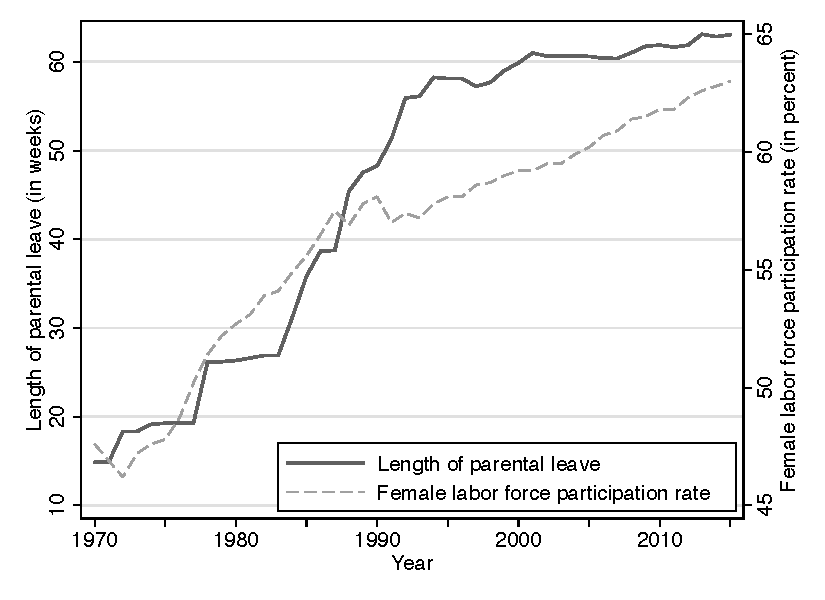
\includegraphics[width=0.8\textwidth]{../analysis/graphs/SOEP/PL_OECD.pdf}
\caption{Own illustration: average length of parental leave and female labor force participation rate across OECD countries}\vspace{-0.3cm}
\begin{minipage}{\textwidth} % choose width suitably
{\footnotesize \textit{Source: }OECD}
\end{minipage}
\end{figure}

\end{frame}
%------------------------------------------------------
\begin{frame}
\begin{block}{Goals: Leave mandates}
\begin{itemize}
\item focus on child care $\rightarrow$ support child development
\item prevent damages to health of mother or child
\item protection against job dismissal
\item compensate income losses $\rightarrow$ secure standards of living
\end{itemize}
\end{block}\pause

\begin{block}{Large transfer payments}
\begin{itemize}
\item German ministry of family affairs:\newline $6$ billion Euros for 2016 ($\sim2\%$ entire federal government budget)
\end{itemize}
\end{block}

\end{frame}
%------------------------------------------------------
\begin{frame}{\mbox{Evaluation: 1979 Reform in West Germany}}
\textbf{$\Rightarrow$ What are the causal effects of the length of maternity leave on children's health in the long-run?}
\medskip
\only<2>{
\begin{columns}
	\begin{column}{.6\textwidth}
		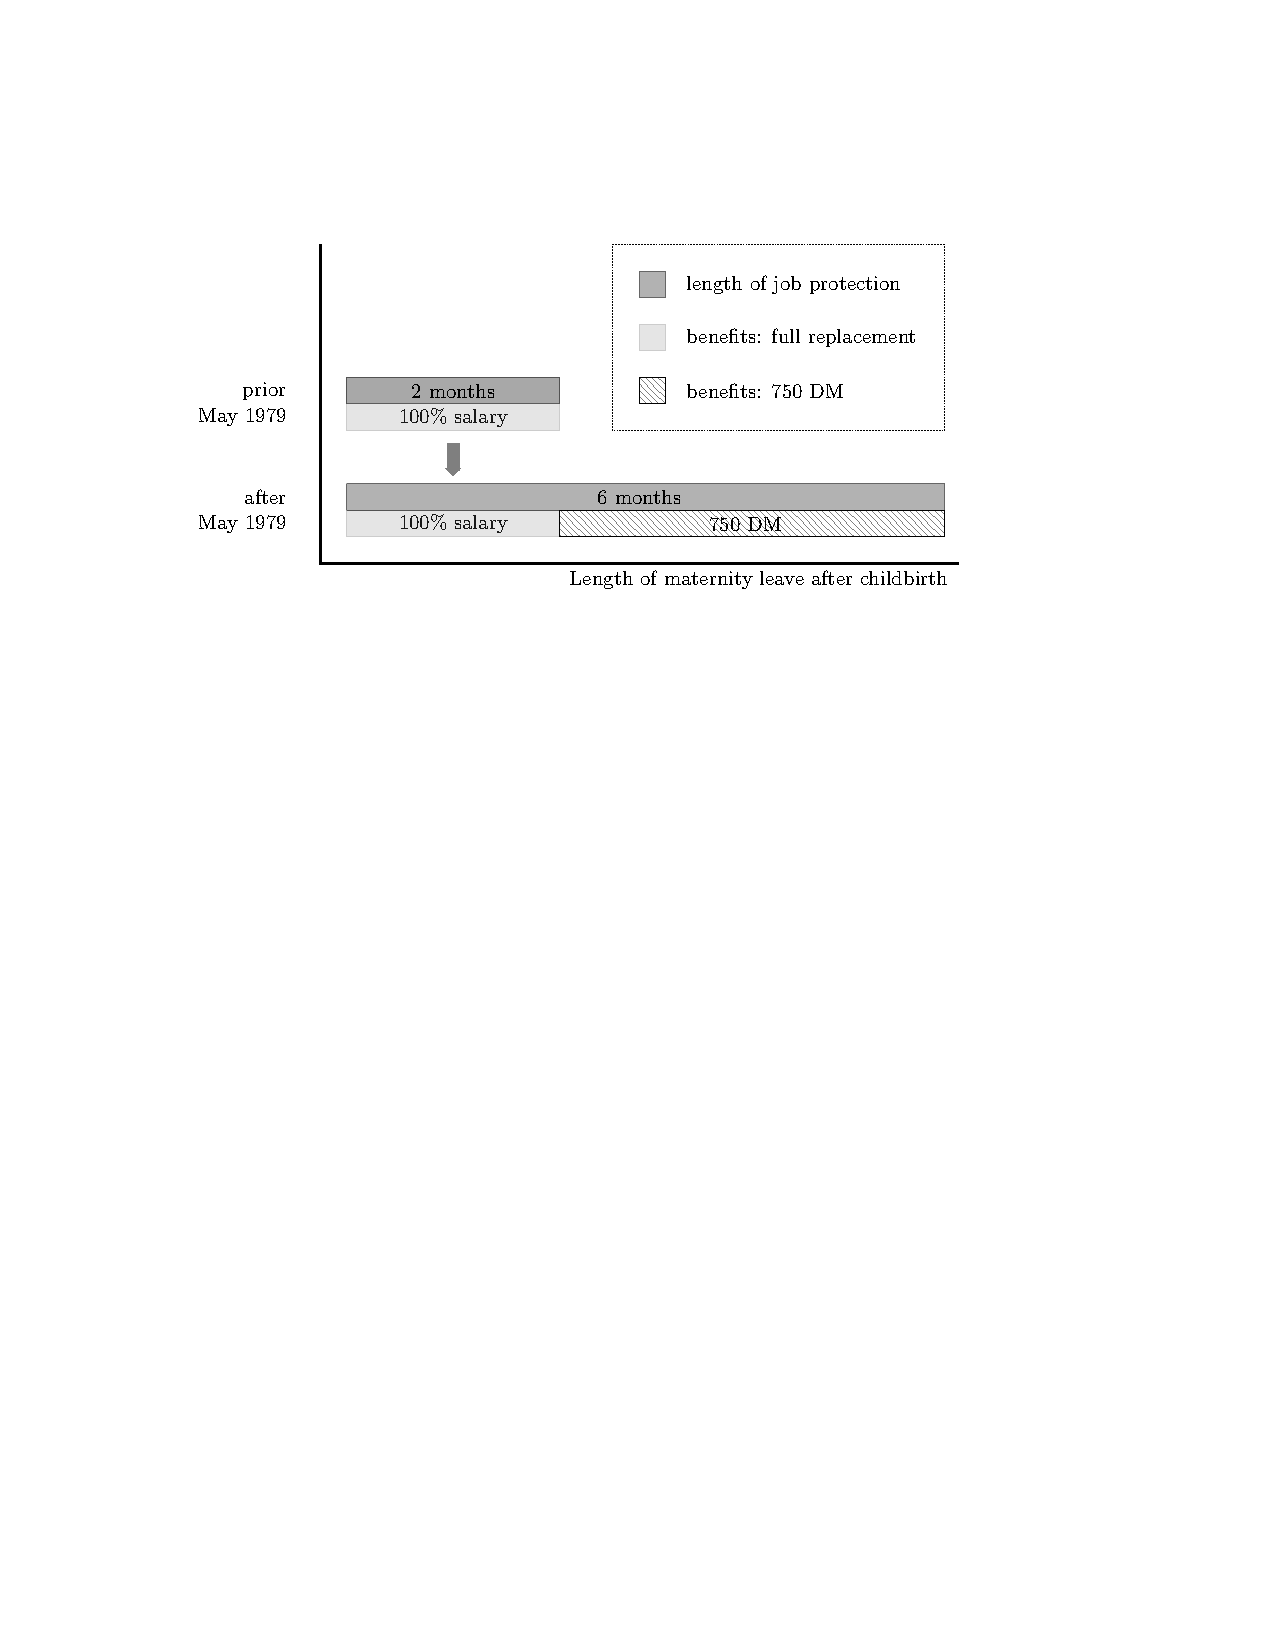
\includegraphics[width = \textwidth]{../analysis/graphs/SOEP/Reform_shortened.pdf}
	\end{column}%
	\begin{column}{.40\textwidth}\small
		\textbf{Exogenous variation in maternity leave:}\newline \begin{itemize}
		\item Extension in paid leave by four months
		\item Universal eligibility for working women
		\item First stage: Maternal labor supply is reduced by 0.835 months
		\end{itemize}
	\end{column}%
	\hfill
	
\normalsize
\end{columns}}
\end{frame}
%------------------------------------------------------
\begin{frame}
\begin{block}{Channels: Length of ML $\rightarrow$ LR child health outcomes?}
\begin{enumerate}
\item \textbf{Higher quality care/more maternal time} 
\begin{itemize}
\item[-]Breastfeeding (Baker and Milligan, 2008)
\begin{itemize}
\item medical advantages (Horta et al., 2007)
\item stronger mother-child linkages $\rightarrow$ crucial for cognitive development (Klaus, 1998); associated with less behavioral problems (Brooks-Gunn et al., 2002)
\end{itemize}
\item[-]Better monitor child's health status and more timely doctor visits (Berger et al., 2005)

\item[-] Prepare healthier meals and lower risk of injuries and infectious disease (Morrill, 2011)\pause
\end{itemize}


\item \textbf{Changes in HH income}
\begin{itemize}
\item[-] transitory  shocks do not affect child development (Carneiro et al., 2017).
%\item association with educational attainment (Dahl and Lochner, 2012) \& child health (Hoynes et al., 2015)
%\item reduced income share $\rightarrow$ expenditure for child goods (Lundberg and Pollak, 1996)
\end{itemize}\pause
\item \textbf{Changes in parental health outcomes}, e.g. stress, depression, poor health $\rightarrow$ affect ability to nurture (Beuchert et al., 2014)\pause
\item \textbf{Effects on higher-order fertility} (Lalive and Zweimüller, 2009); quantity of children and birth spacing
\end{enumerate}
\end{block}
\end{frame}




%------------------------------------------------------
%\begin{frame}
%\begin{block}{OLD!!!!!!! Channels: Length of ML $\rightarrow$ LR child health outcomes?}
%\begin{enumerate}
%\item \textbf{Higher quality care, e.g. breastfeeding} (Baker and Milligan, 2008; Berger et al., 2005)
%\begin{itemize}
%\item medical advantages (Horta et al., 2007)
%\item stronger mother-child linkages $\rightarrow$ crucial for cognitive development (Klaus, 1998)
%\end{itemize}\pause
%\item \textbf{Changes in HH income}
%\begin{itemize}
%\item association with educational attainment (Dahl and Lochner, 2012) \& child health (Hoynes et al., 2015)
%\item reduced income share $\rightarrow$ expenditure for child goods (Lundberg and Pollak, 1996)
%\end{itemize}\pause
%\item \textbf{Changes in parental health outcomes}, e.g. (stress, depression, poor health) (Beuchert et al., 2014)\pause
%\item \textbf{Effects on higher-order fertility} (Lalive and Zweimüller, 2009); quantity of children and birth spacing
%\end{enumerate}
%\end{block}



%$\Rightarrow$ Only parental perspective. Later, I investigate children's adulthood labor market, education and family outcomes as potential pathways

%\end{frame}


\begin{frame}{Literature}
\textbf{Previous Literature:}
\begin{enumerate}
\item \underline{Long-term effects of parental leave}\\ Inconclusive and more emphasis on educational attainment and labor market outcomes
\item \underline{Parental leave $\rightarrow$ health (both maternal and infant)} \\only short-run effects
\end{enumerate}\pause
\bigskip
$\Rightarrow$ \textbf{Contribution to the literature:}
\begin{itemize}
\item Adding to the scarce evidence of health outcomes, in particular in the long-run

\item Causal ITT effects of maternity leave in the first year based on large administrative data sets

\item Comprehensive analysis: broad range of health outcomes 

%\item life-course approach applied in complete new setting 

%\item identification strategy $\rightarrow$ less dependence on identifying assumptions

%\item In progress: usage of special datasets
\end{itemize}
\end{frame}
%------------------------------------------------------



%-=-=-=-=-=-=-=-=-=-=-=-=-=-=-=-=-=-=-=-=-=-=-=-=
%	IDENTIFICATION STRATGEY:
%-=-=-=-=-=-=-=-=-=-=-=-=-=-=-=-=-=-=-=-=-=-=-=-=
\section{Identification}
%------------------------------------------------------
\begin{frame}{Difference-in-Difference Regression Discontinuity (DD-RD)}
Estimation strategy following Dustmann and Schönberg (2012): eradicate season-of-birth effects
\begin{align*}
\resizebox{.99 \textwidth}{!} 
{$Y_{imt} = \gamma_0 + \gamma_1 T_{im} + \gamma_2 After_{im}+ \color{red}\gamma_3 \color{black}T_{im} \times After_{im} +  Z_{imt}' \delta + \sum_{m} \psi_m D_{im} +\xi_{imt} $}%\label{eq:RD+DD}
\end{align*}
\vspace{-0.5cm}
\begin{itemize}
\begin{scriptsize}
\item[-] $Y_{imt}$: number of diagnoses divided by number of individuals in respective month-of-birth cohort
\item[-] $T_{im}$: treatment dummy equals one if individual is born in the treatment year
\item[-] $After_{im}$: dummy whether individual is born in/after May
\item[-] $T_{im} \times After_{im}$: interaction equals one for group of interest (born between May-Oct 1979 in the widest specification)
\item[-] $Z_{imt}$: vector of personal background characteristics
\item[-] DD allows to include birth month dummies $D_{im}$
\item[-]local estimation: 2-6 months to the left/right of reform cut-off date
\item[-] \texttt{control} cohort: birth cohort one year prior to the reform
\item[-] Identifying assumption: seasonal part is time-invariant



%\item[-] Intention-to-treat effect

\end{scriptsize}
\end{itemize}
\end{frame}

%------------------------------------------------------

%-=-=-=-=-=-=-=-=-=-=-=-=-=-=-=-=-=-=-=-=-=-=-=-=
%	 DATA & VARIABLES:
%-=-=-=-=-=-=-=-=-=-=-=-=-=-=-=-=-=-=-=-=-=-=-=-=
\section{Data}
\begin{frame}{Data \& Variables}
\textbf{I) Hospital administrative data (2005-2013):} 
\begin{itemize}
\item[-] Universe of German in-patient cases ($\approx 18$ Mio/year). \newline Information about patient's main diagnosis, age, gender, place of residence, date of admission and discharge.
\item[-] Outcomes: admission, severity measures, mental and behavioral disorders, digestive \& circulatory system
\end{itemize}


\pause
 \textbf{II) German Micro Census (2005-2013):}
\begin{itemize}
\item[-] Europe's largest household survey ($1\%$ of German population), contains information on educational attainment, employment status, income as well as health information
\item[-] Outcomes: Overweight, legally handicapped, sickness, hospital admission

\item[-]Advantage: only individuals whose mothers were affected by reform (foreign-born children and children born in the GDR eliminated from analysis)

\end{itemize} 
 

\end{frame}
%------------------------------------------------------

%\begin{frame}{Data}
%German Socio Economic Panel (1993-2014)
%\begin{itemize}
%\item only individuals whose mothers were affected by reform (foreign-born children and children born in the GDR eliminated from analysis)
%\item drawback: compared to other studies, small sample size
%\item advantages
%\begin{enumerate}
%\item Possibility link children to their parents
%\item One of longest running HH surveys $\rightarrow$ extensive window of longitudinal observations
%\end{enumerate}
%\item working data set: 
%\begin{table}
%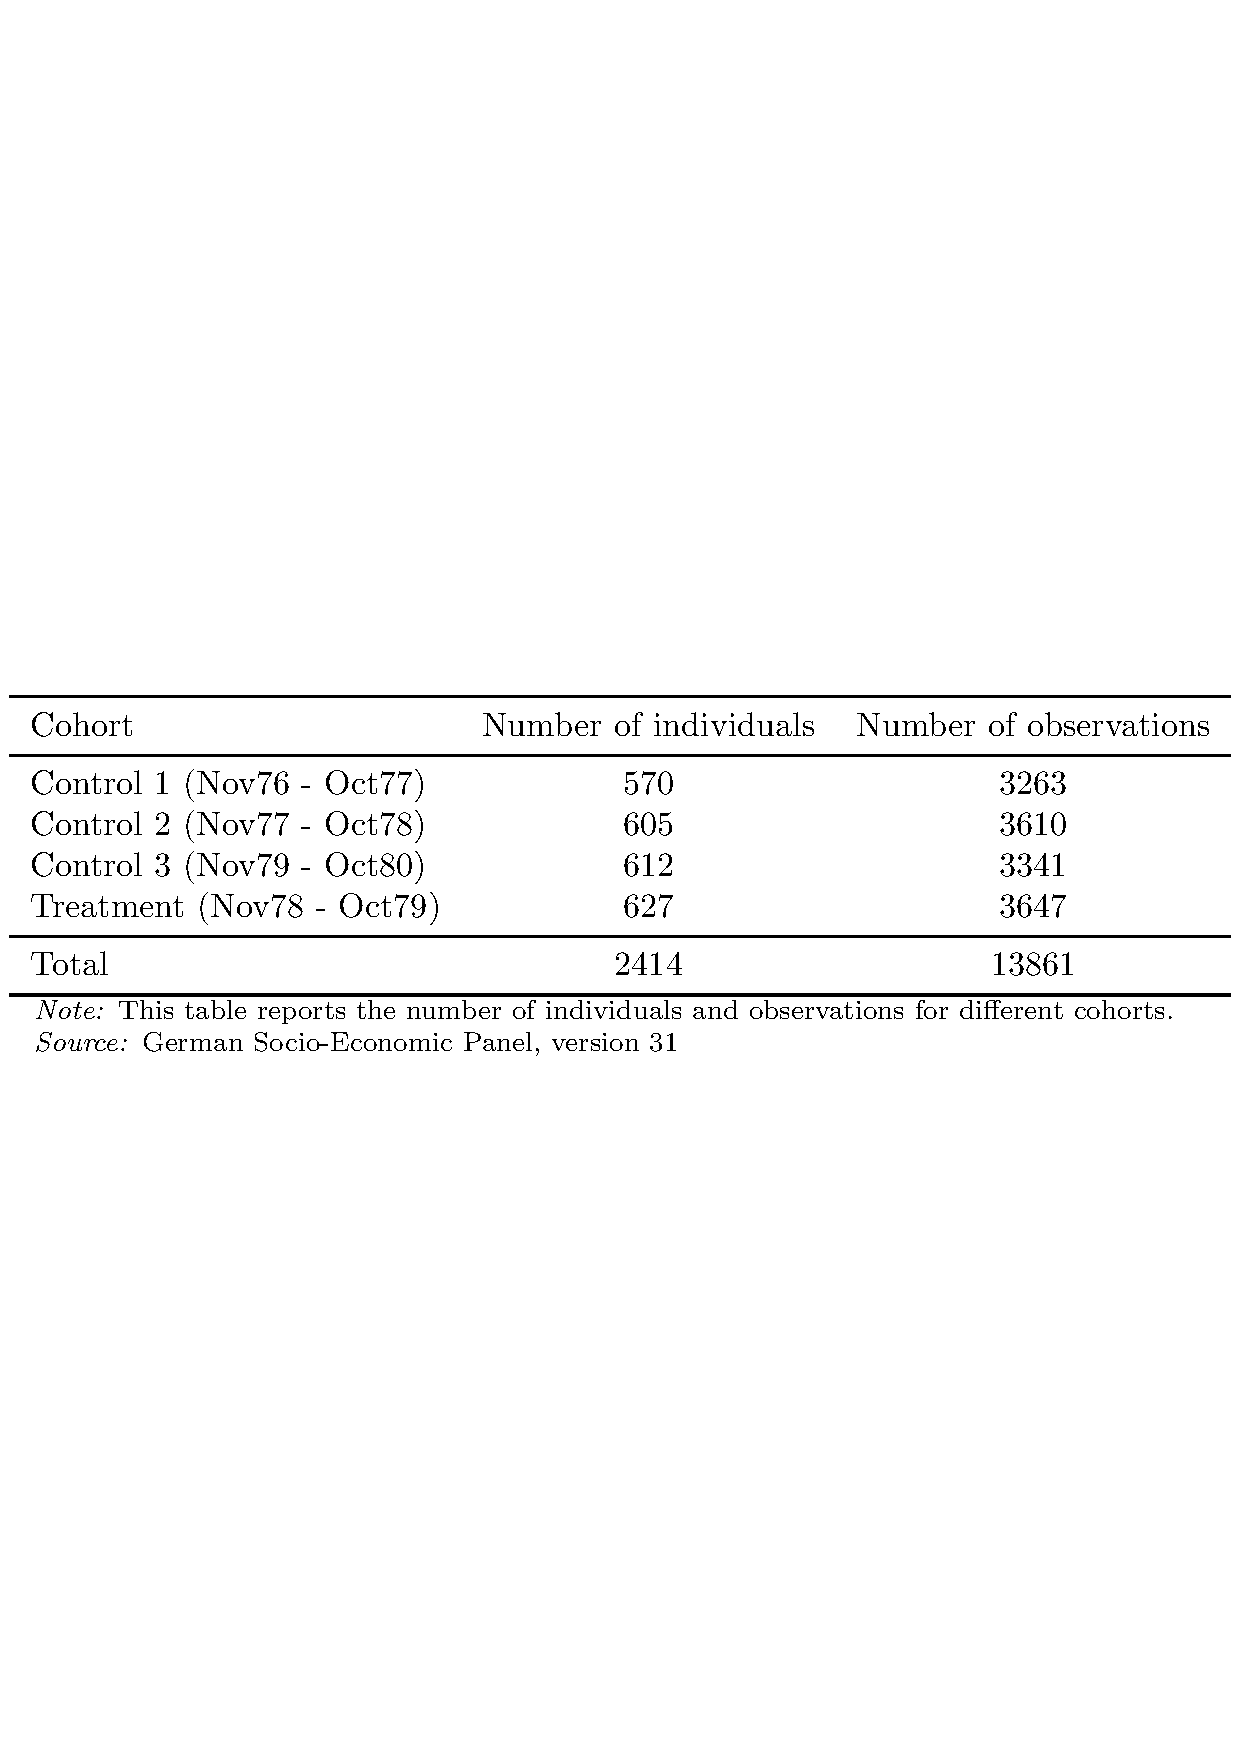
\includegraphics[width=0.8\textwidth]{presentation/data}
%\caption{Number of observations, per cohort}
%\end{table}
%\end{itemize}
%\end{frame}
%%------------------------------------------------------
%\begin{frame}{Variables}
%\underline{Wide variety of health outcome variables}
%\begin{itemize}
%\item \textbf{Subjective Outcomes:} Self-assessed health and sleep, concerns about own health, problems with carrying out daily tasks, ability to handle stress, experienced pain recently, constrained in social life\pause
%\item \textbf{Biometric Outcomes:} Weight, height, BMI, overweight and obesity
%\item \textbf{Objective Outcomes:} Sickness\footnotemark[1], doctor visits\footnotemark[1], hospitalization, disability, illness, chronic disease
%\item \textbf{Health behavior:} follow healthy diet, smoking\footnotemark[1], alcohol, private health insurance, hours of sleep
%\end{itemize}
%\begin{small}
%\textbf{Personal background characteristics:} sex, age, migration background, marital status, children, employment status, inflationary adjusted annual HH income, schooling
%\end{small}
%\footnotetext[1]{Both at the extensive and intensive margin.}
%\end{frame}
%------------------------------------------------------


%-=-=-=-=-=-=-=-=-=-=-=-=-=-=-=-=-=-=-=-=-=-=-=-=
%	 ANALYSIS
%-=-=-=-=-=-=-=-=-=-=-=-=-=-=-=-=-=-=-=-=-=-=-=-=
\section{Analysis}
\subsection{Validity}
%------------------------------------------------------
\begin{frame}{Validity}
Problem: Behavioral responses with respect to the running variable. Is birth a random variable $\sim$ $\mathcal{N}(40w,2w)$?\pause
\begin{itemize}
\item \textbf{Strategic conception}\newline draft bill does not allow to react to reform (4 months before reform put into practice), media coverage (earliest 2 months)

\item \textbf{Postponing induced births and cesarean sections}\newline Gans \& Leigh (2009): Australian baby bonus\newline $\rightarrow$ similar distortionary ”introduction effects”?\pause



\begin{enumerate}
\item Timing of birth $\rightarrow$ fertility distribution
\item Parental pre-determined covariate balance
\end{enumerate}
\end{itemize}\pause
\medskip
$\Rightarrow$ No indication of sorting, occurrence of birth is a random event; policy change can be seen as true quasi-experiment \newline $\Rightarrow$ Additional robustness check: Donut specification
\end{frame}
%------------------------------------------------------
% ALL YEARS FERTILITY HISTOGRAM
\begin{frame}{Validity II: Fertility distribution}
\begin{figure}
\begin{tikzpicture}
	\node[anchor=south west,inner sep=0] at (0,0) {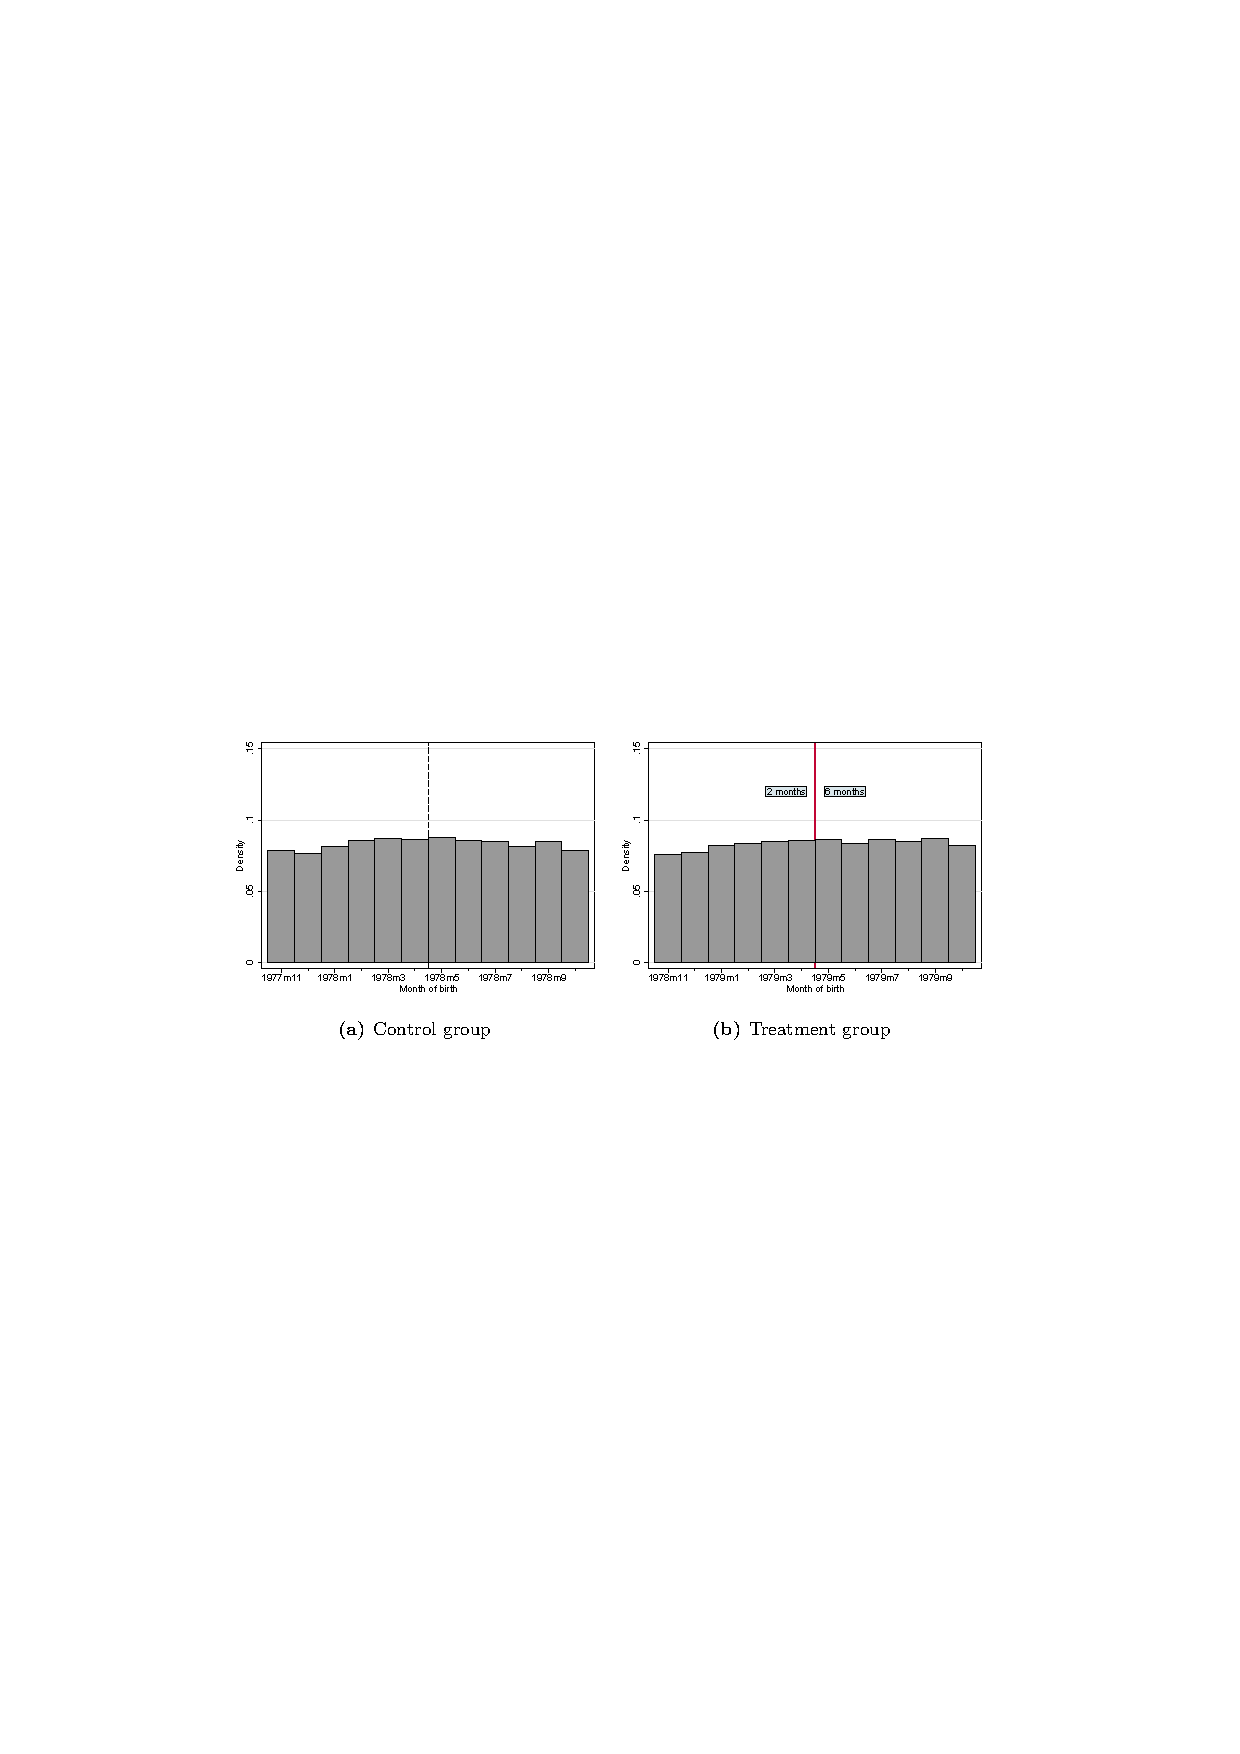
\includegraphics[width=0.99\textwidth]{../analysis/graphs/presentation/fertility}};
	%\draw[red,ultra thick,rounded corners] (5.2,0) rectangle (10.3,4.3);
	\end{tikzpicture}
\end{figure}
\begin{center}\vspace{-1em}
\tiny \flushleft Note:  The figures display the relative frequency of birth months per birth cohort, adjusted for different lengths of the months.  Source: Destatis.
\end{center}
\end{frame}
%------------------------------------------------------
% PARENTAL COVARIATE BALANCE TABLE
\begin{frame}{Validity III: Balancing table}
\begin{figure}
\textbf{Pre-determined covariate balance}
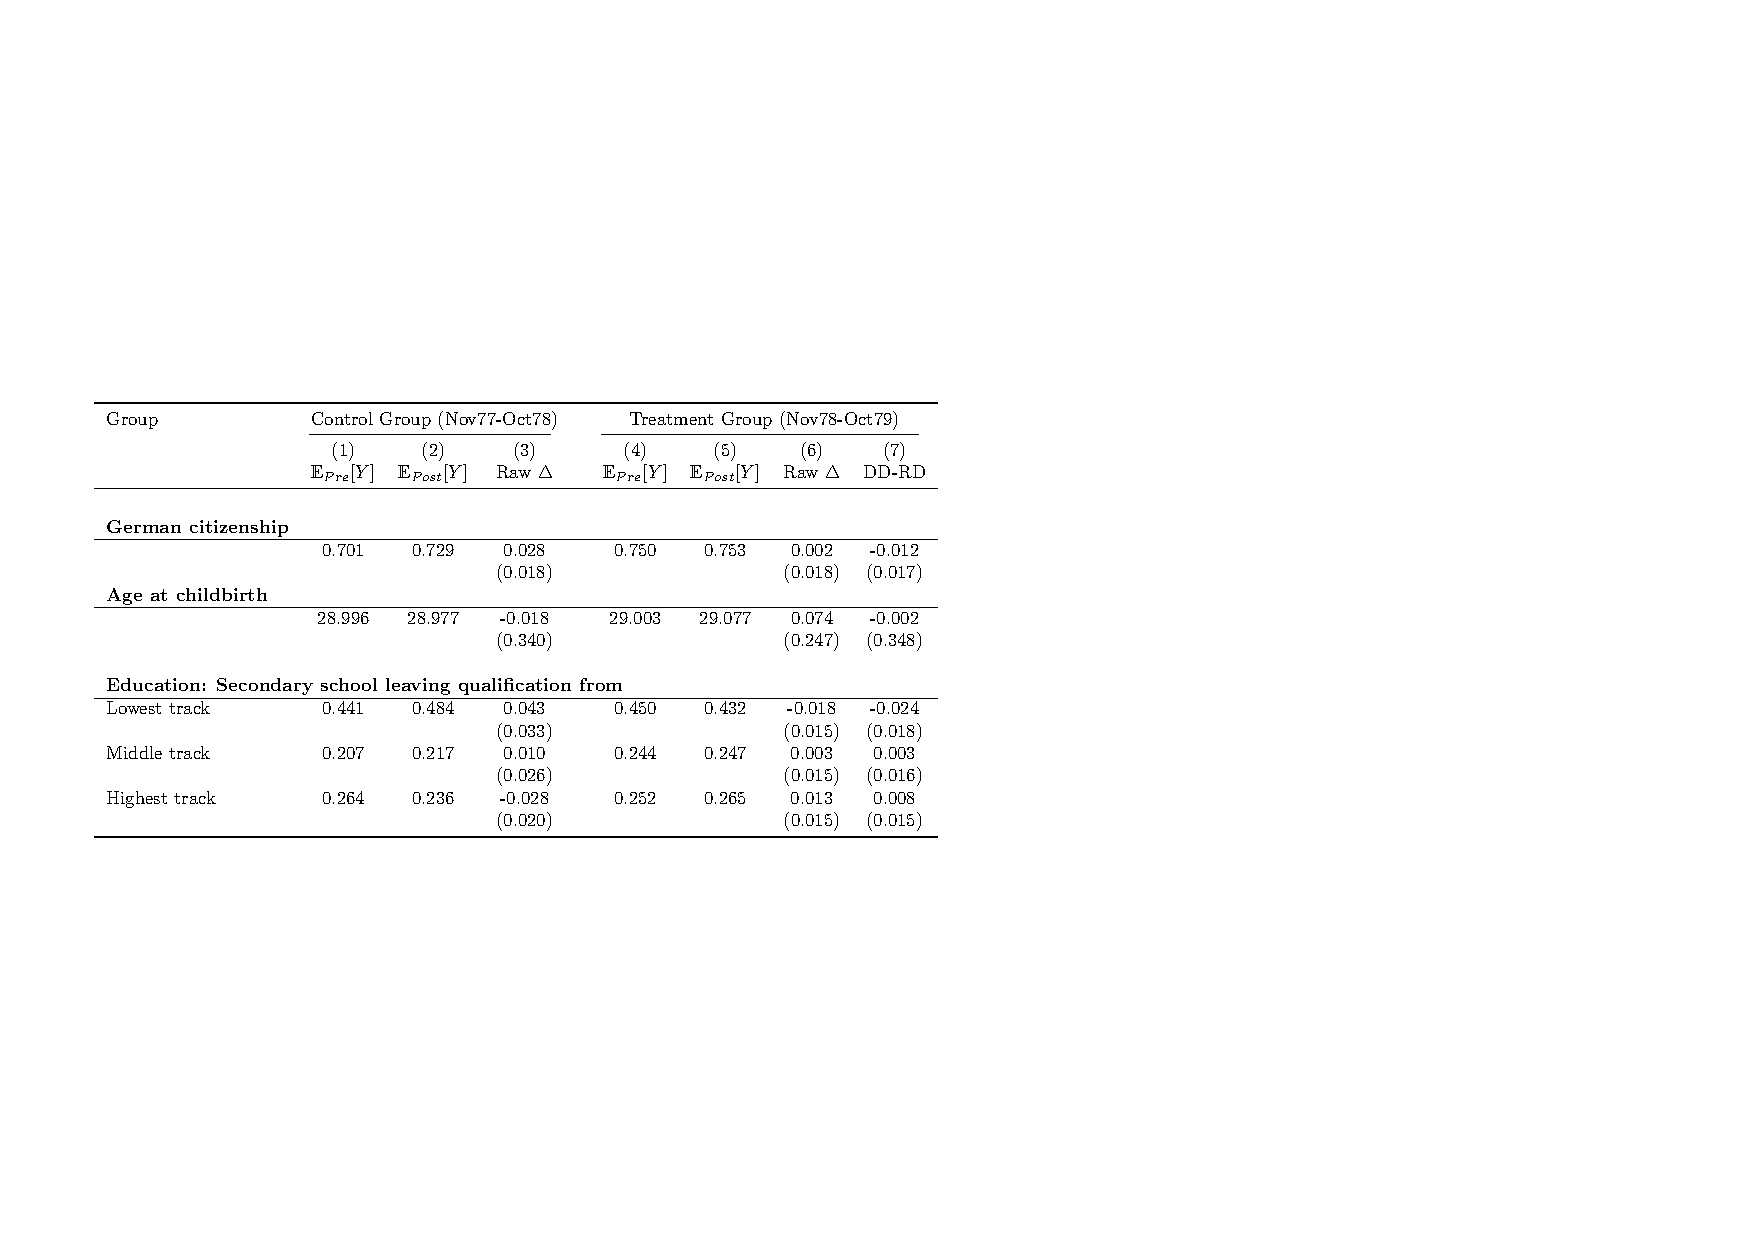
\includegraphics[width=0.9\textwidth]{../analysis/graphs/presentation/parental_covariate_balance}
\end{figure}
\begin{minipage}{1.0\linewidth}
\begin{center}\vspace{-1cm}
\tiny \flushleft Note: The table compares parental characteristics within half a year around the threshold. It reports difference-in-means and DD-RD estimates. Source: German Micro Census, waves 2005, 2009 and 2013. 
\end{center}
\end{minipage}


\end{frame}
%------------------------------------------------------



%%%%%%%%%%%%%%%%%%%%%
% KKH DIAGNOSEDATEN
%%%%%%%%%%%%%%%%%%%%%
\subsection{Results}
%hauptttabelle
\subsection{a) Hospital registry data}
\begin{frame}{(1) Results from the hospital registry data (pooled)}

%\begin{block}{Pooled:}
\begin{figure}
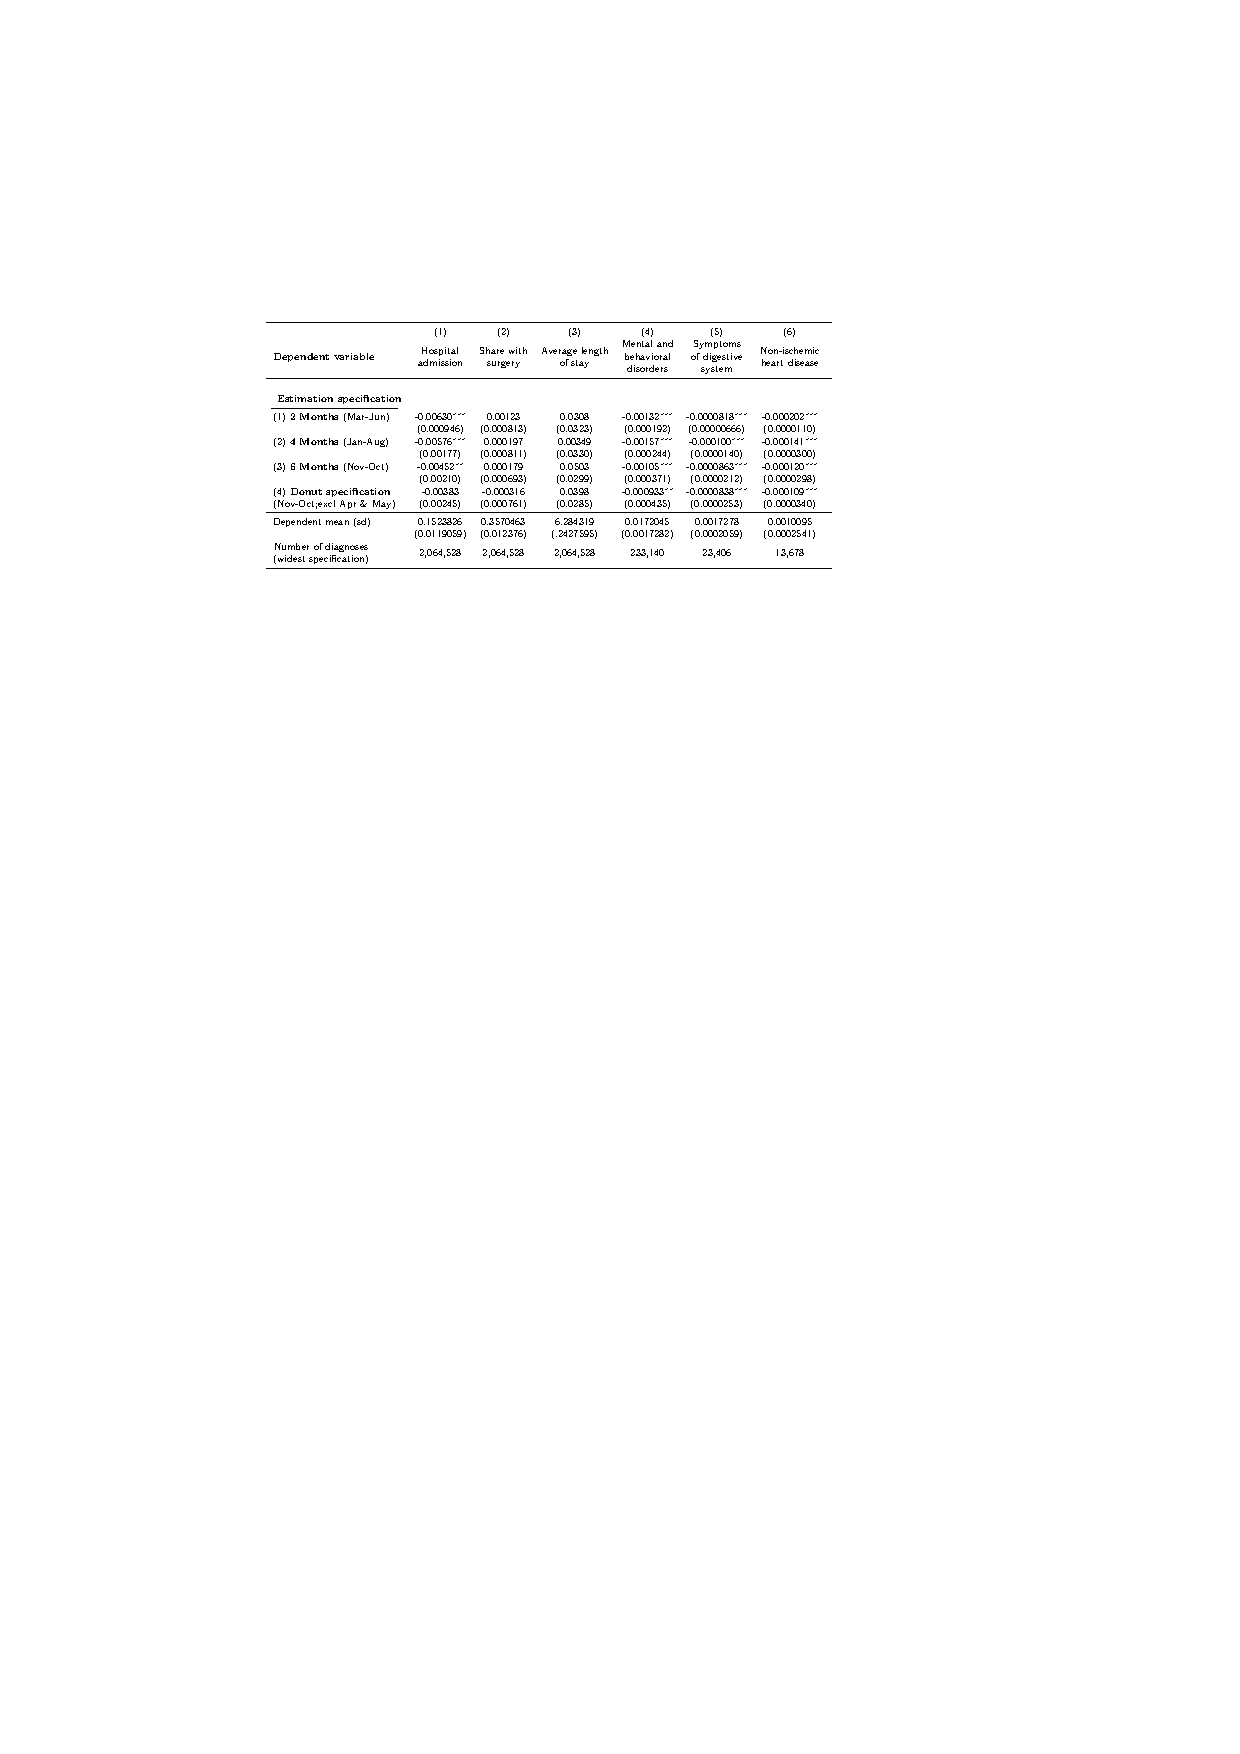
\includegraphics[width = 1.0\linewidth]{../analysis/graphs/KKH/outcome_v2.pdf}
\end{figure}
%\end{block}
\begin{center}
\vspace{-0.5em}
\tiny \flushleft Note: This table reports various DD-RD estimates of the impact of the expansion of maternity leave from two to six months on different sets of health outcomes. The estimates are based on equation 1. The control group is comprised of children that are born in the same months but one year prior the reform (i.e. children born between  November 1977 and October 1978). The outcomes are measured over the period 2005-2013. Clustered standard errors are reported in parentheses. Significance levels: * \(p<0.10\), ** \(p<0.05\), *** \(p<0.01\).\newline Source: German hospital administrative data. 
\end{center}

\end{frame}
%------------------------------------------------------
\begin{frame}{(2) Life-cycle perspective}
\begin{figure}[p]
%LIFECOURSE PERSPECTIVE
\begin{subfigure}[h]{0.45\textwidth}\centering
	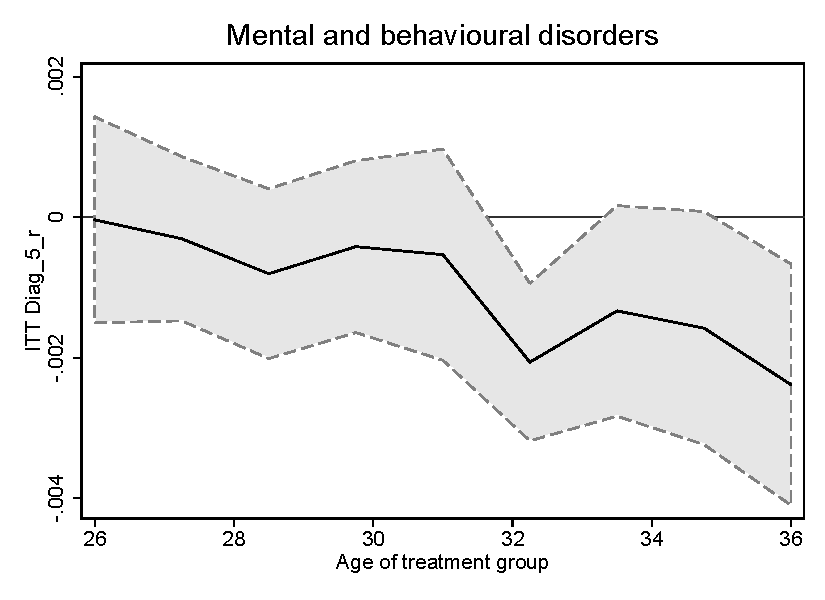
\includegraphics[width=\textwidth]{../analysis/graphs/KKH/R1_LC_Diag_5_r}
\end{subfigure}
\quad
\begin{subfigure}[h]{0.45\textwidth}\centering
	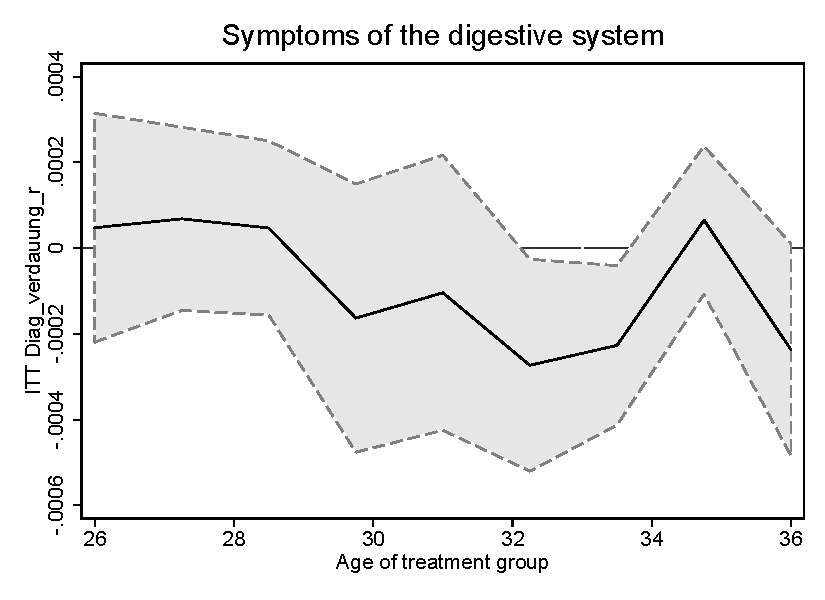
\includegraphics[width=\textwidth]{../analysis/graphs/KKH/R1_LC_Diag_verdauung_r}
\end{subfigure}
\begin{subfigure}[h]{0.45\textwidth}\centering
	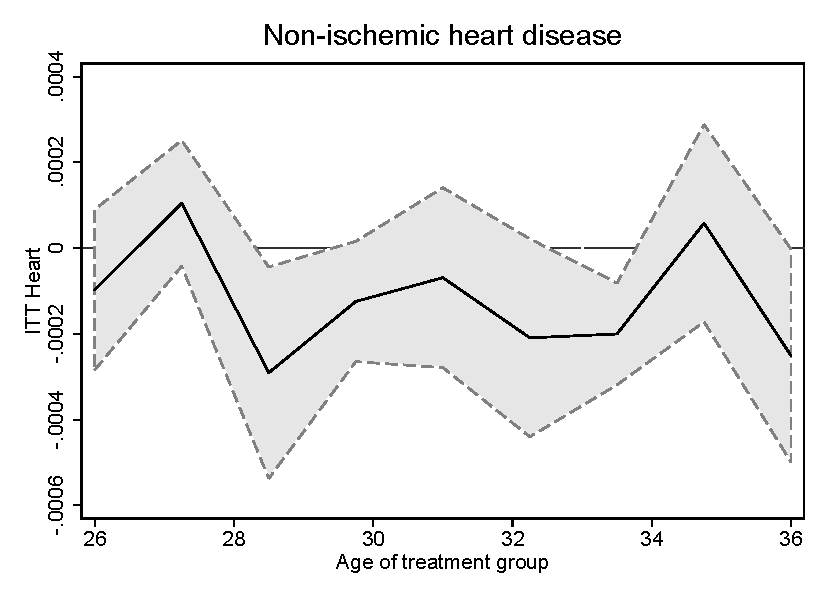
\includegraphics[width=\textwidth]{../analysis/graphs/KKH/R1_LC_Heart}
\end{subfigure}
\quad
\begin{subfigure}[h]{0.45\textwidth}\centering
	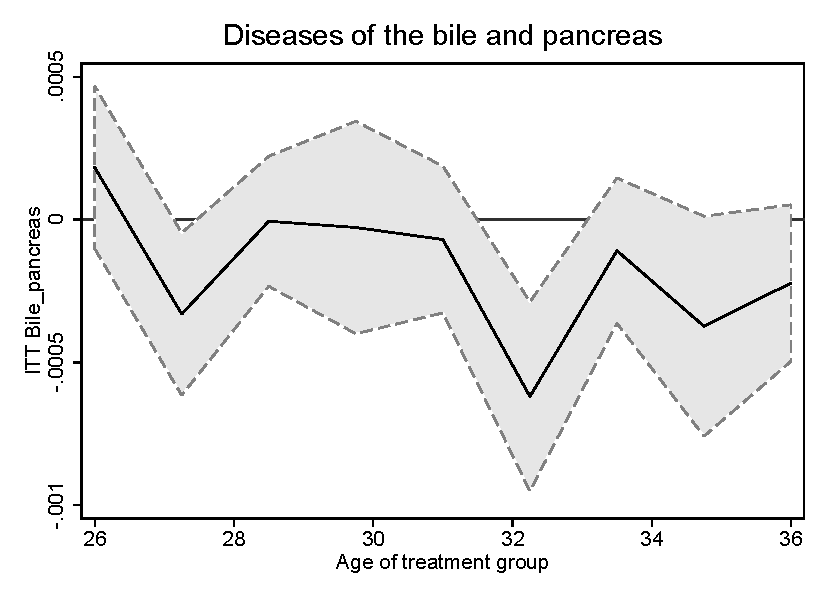
\includegraphics[width=\textwidth]{../analysis/graphs/KKH/R1_LC_Bile_pancreas}
\end{subfigure}
\end{figure}
\begin{minipage}{0.95\linewidth}
\tiny \flushleft Note: The figures plot various DD-RD estimates (along with 90\% confidence intervals) of the impact of the expansion of maternity leave from two to six months on different sets of health outcomes. Estimates come from a regression based on equation (1), which are run separately for each age value.
\end{minipage}
\end{frame}

%%%%%%%%%%%%%%%%%%%%%
% MIKROZENSUS
%%%%%%%%%%%%%%%%%%%%%
\subsection{b) Micro Census}
\begin{frame}{\mbox{(3) Results from the German Micro Census}}
\begin{figure} \begin{center}
\textbf{Health outcomes}
\end{center} 
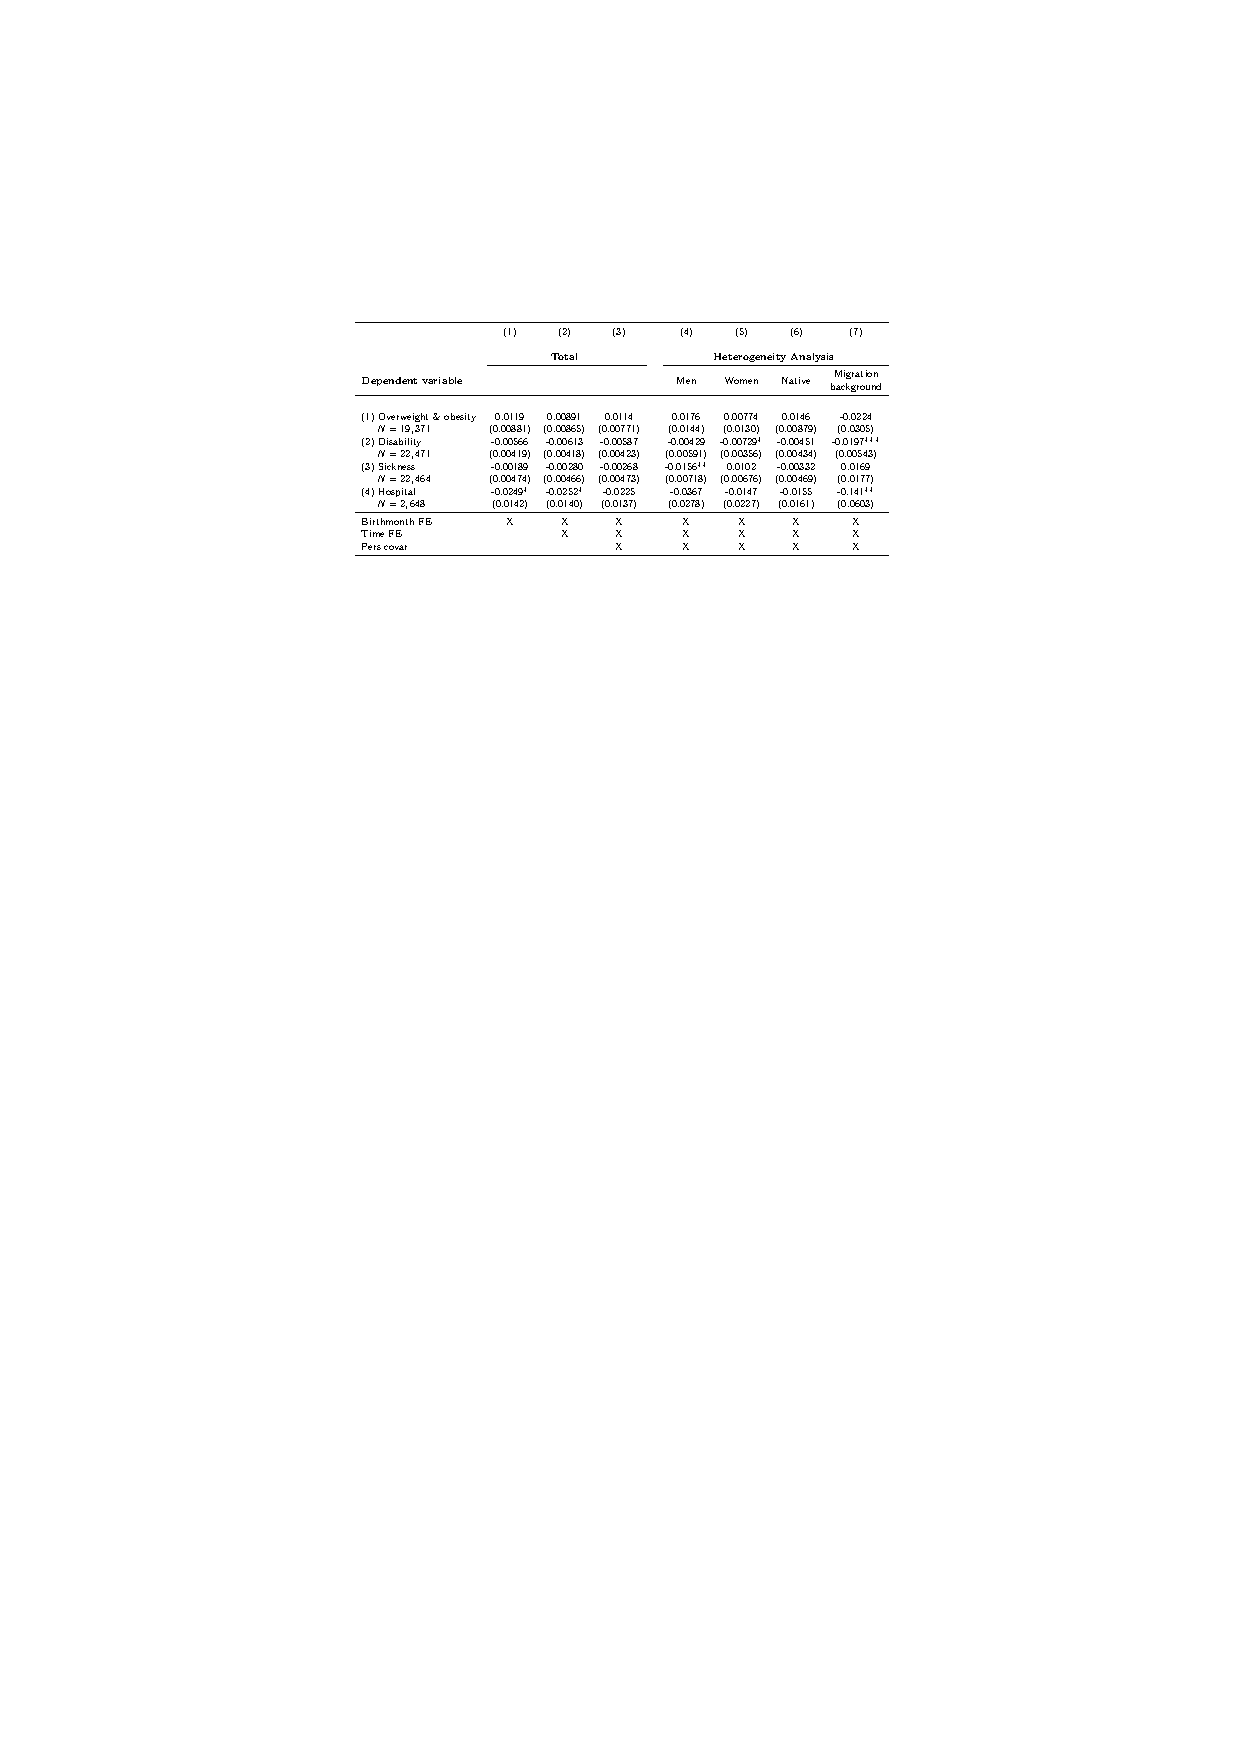
\includegraphics[width = 0.99\linewidth]{../analysis/graphs/KKH/outcome_MZ_health.pdf}
\end{figure}\vspace{-2.5em}
\tiny \flushleft Note: This table reports various DD-RD estimates of the impact of the expansion of maternity leave from two to six months on different sets of health outcomes. The estimates are based on equation 1. The control group is comprised of children that are born in the same months but one year prior the reform (i.e. children born between  November 1977 and October 1978). Clustered standard errors are reported in parentheses. Significance levels: * \(p<0.10\), ** \(p<0.05\), *** \(p<0.01\).\newline Source: German Micro Census, waves 2005, 2009 and 2013). 
\end{frame}
%------------------------------------------------------
%SES OUTCOMES
\begin{frame}{(4) Causal effects on socio-economic outcomes}
\begin{figure}
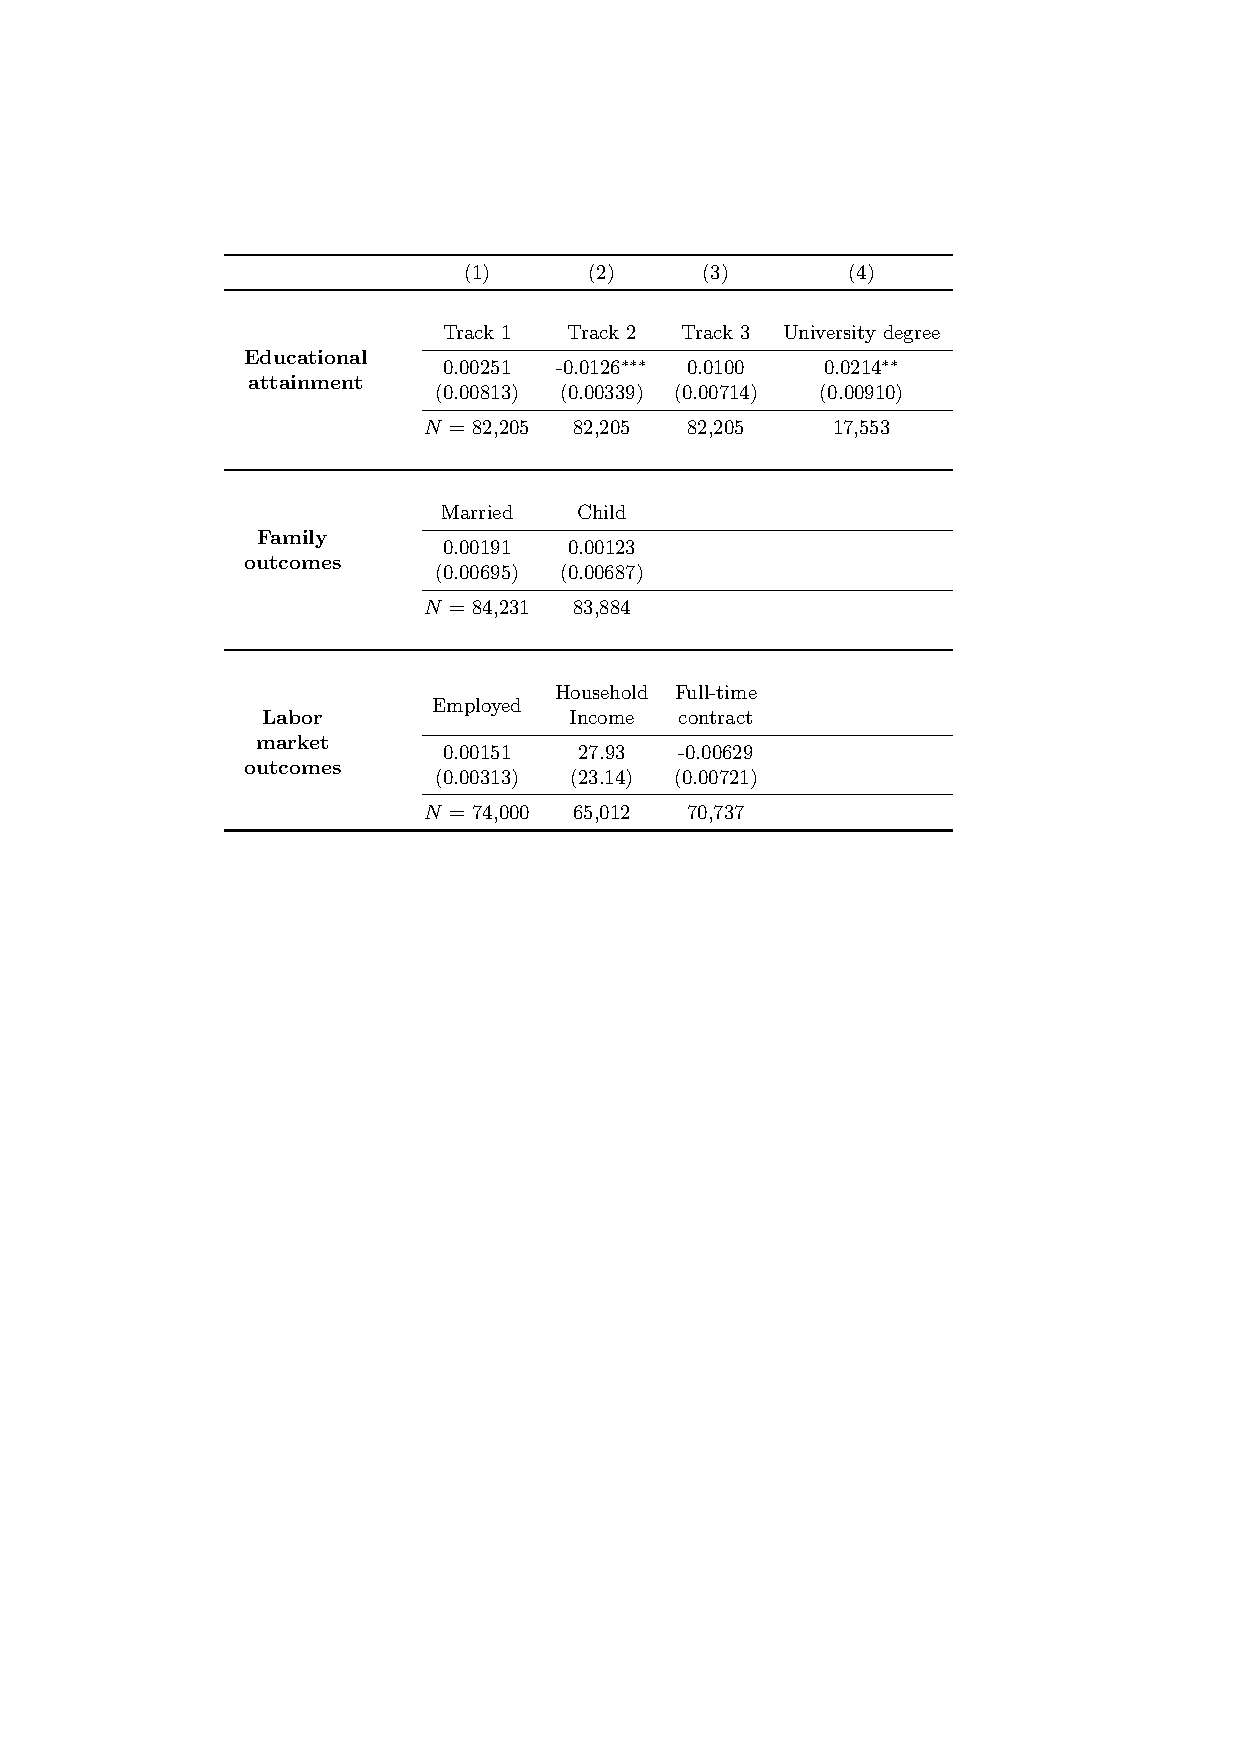
\includegraphics[width=0.8\linewidth]{../analysis/graphs/presentation/ses_outcomes}
\end{figure}
\vspace{-1.35em}
\tiny \flushleft Note: This table reports various DD-RD estimates of the impact of the expansion of maternity leave from two to six months on different sets of socio-economic outcomes.  Clustered standard errors are reported in parentheses. Significance levels: * \(p<0.10\), ** \(p<0.05\), *** \(p<0.01\). Source: German Micro Census, waves 2005-2013). 
\end{frame}


	

%------------------------------------------------------
%\begin{frame}{(4) Heterogeneity analysis}
%\textbf{Do subgroups react differently to reform?}\newline
%\label{BACK_HETERO}
%\begin{itemize}
%\item Effects of reform are worse for \begin{itemize}
%\item males
%\item  individuals whose parents have a school certificate from the lowest track
%\end{itemize}
%\item Migration background does not seem to matter that much
%\end{itemize}
%\bigskip\bigskip\bigskip
%
%
%
%
%
%
%
%
%\hyperlink{MECHANISMS}{\beamerbutton{Mechanisms}}


%
%
%\begin{columns}
%	\begin{column}{.50\textwidth}
%		\textbf{Health maps:}\newline
%$\rightarrow$ positive impacts of ML in economically strong federal states and vice versa
%	\end{column}%
%	\hfill
%	
%\begin{column}{.48\textwidth}
%		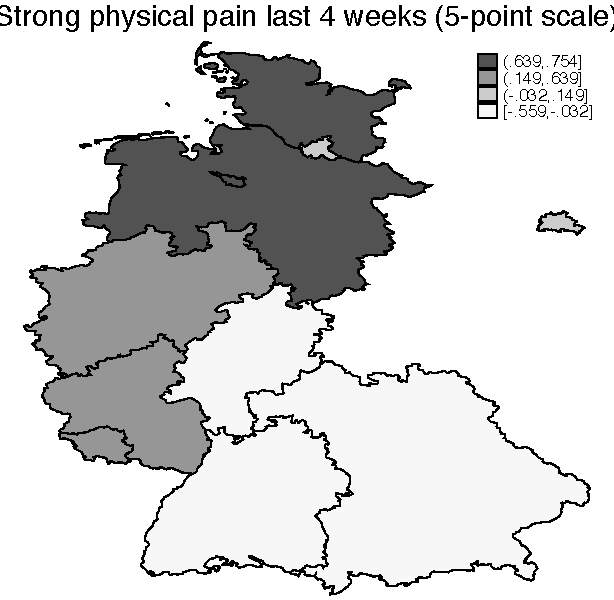
\includegraphics[height=4cm]{LOCPhys_pain.pdf}
%\end{column}%
%	
%\end{columns}



%\end{frame}


%------------------------------------------------------
%\begin{frame}{(5) Mechanisms}
%SES health gradiant: use SES $\rightarrow$ health for potential pathways
%\begin{enumerate}
%\item educational attainment: insignificant 
%\item family outcomes: more likely to have children\footnotemark[4]
% and being married\footnotemark[4]
%\item labor market outcomes: more likely to be unemployed and lower HH labor income\footnotemark[4]
%\end{enumerate}
%
%
%\textbf{Take-away:}
%\begin{itemize}
%\item $\Rightarrow$ \mynum{1} and \mynum{3} are verified by Dustmann and Schönberg (2012)
%\item \mynum{1} excluded, \mynum{3} possible explanation, \mynum{2} ambiguous effect
%\item Merely suggestive evidence
%\end{itemize}
%
%
%\footnotetext[4]{Only borderline significant at a 15\% level.}
%\end{frame}

%------------------------------------------------------
% ROBUSTNESS SECTION
\subsection{Robustness}

\begin{frame}{Robustness}

\begin{enumerate}
\item \textbf{Inclusion of covariate vector $Z_{imt}$:} control for compositional changes between \texttt{treatment} and \texttt{control} group 
\item \textbf{Different bandwidths $h$ and Donut specification:} verification that results are not biased by endogenous timing of birth $\rightarrow$ exclude children born in months around threshold
\item \textbf{Choice of control group:} 
\begin{itemize}
\item Additional control cohorts \& various compositions
\item Placebo treatments
\end{itemize}
\end{enumerate}

$\Rightarrow$ Effects on health outcomes are driven by the legislation change in maternity leave

\end{frame}




%-=-=-=-=-=-=-=-=-=-=-=-=-=-=-=-=-=-=-=-=-=-=-=-=
%	 SUMMARY
%-=-=-=-=-=-=-=-=-=-=-=-=-=-=-=-=-=-=-=-=-=-=-=-=
\section{Conclusion}
\begin{frame}{Concluding remarks}
\begin{itemize}
\item \textbf{Points of concern:}
\begin{enumerate}
\item Eligibility universal, but take-up not (40\%) $\rightarrow$ selection on unobservables?
\item Coincidence with peak of second oil crisis, macroeconomic situation at time of conception matters (Dehejia and Lleras-Muney, 2004) $\rightarrow$ one cohort significantly different affected than the other?
\end{enumerate}
\item \textbf{Summary:}
\begin{itemize}
\item Goal of ML: improve welfare of mothers and children
%\item {Large transfer payments involved:} German ministry of family affairs spent $6$ billion Euros in 2016 ($\sim2\%$ entire federal government budget)
\item A large body of the literature does not find effects on other outcomes (SES) - long-run health outcomes have not been in the center of the discussion

\item Previous evidence: no effect of this ML reform on child education and labour market outcomes.
Our results suggest that ML reform had significantly positive effects on child health in the long run.


\end{itemize}
\end{itemize}



\end{frame}




%-=-=-=-=-=-=-=-=-=-=-=-=-=-=-=-=-=-=-=-=-=-=-=-=
%	 THANK YOU
%-=-=-=-=-=-=-=-=-=-=-=-=-=-=-=-=-=-=-=-=-=-=-=-=
\begin{frame}
\begin{center}
Thank you very much for your attention!
\end{center}




\end{frame}

%\section*{Appendix}
%\begin{frame}
%Restlichen Abbildungen, backup slides
%\end{frame}


%-=-=-=-=-=-=-=-=-=-=-=-=-=-=-=-=-=-=-=-=-=-=-=-=
%	 APPENDIX
%-=-=-=-=-=-=-=-=-=-=-=-=-=-=-=-=-=-=-=-=-=-=-=-=
\section*{Appendix}
%------------------------------------------------------
%WORKING DATASET
%\begin{frame}
%\hyperlink{BACK}{\beamerbutton{Back to Data \& Variables}}
%%\begin{table}\label{DATASET}
%%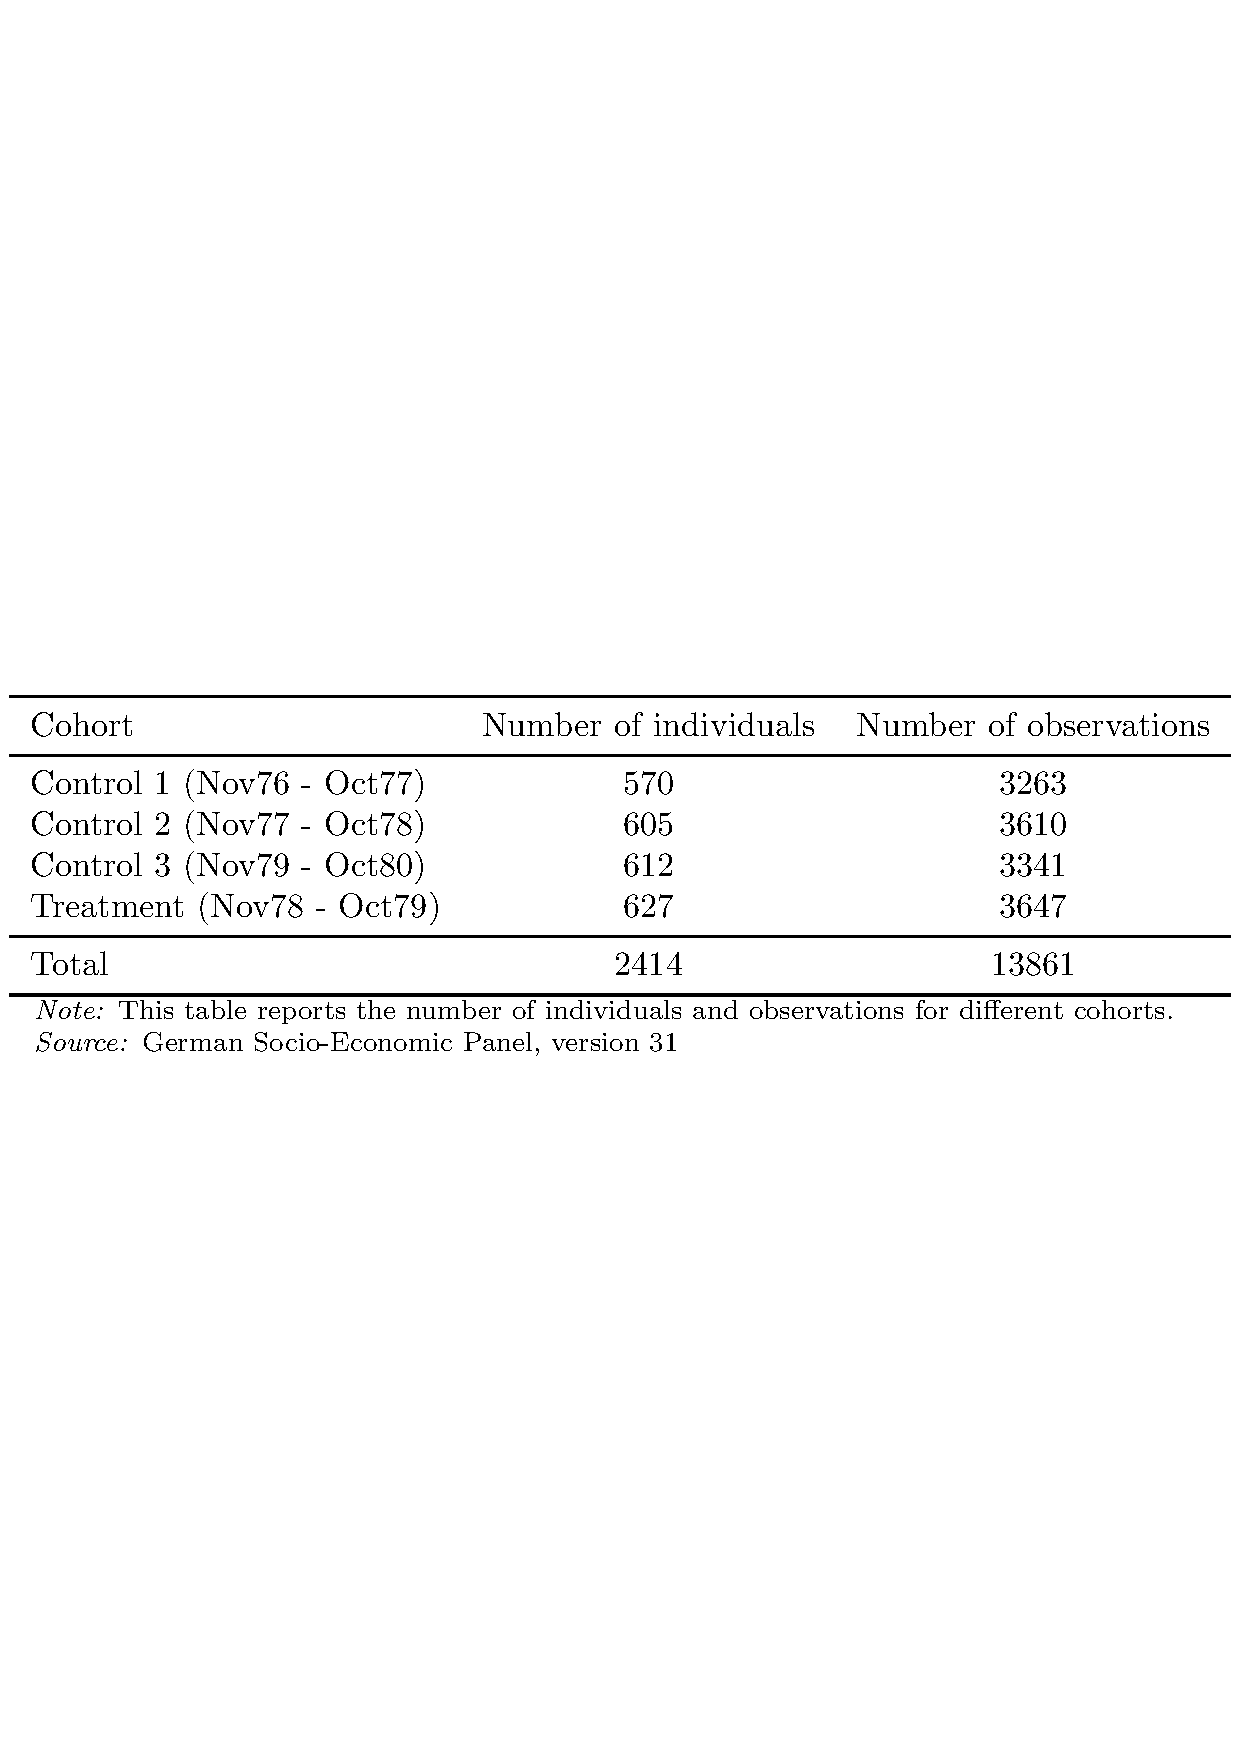
\includegraphics[width=0.8\textwidth]{presentation/data}
%%\caption{Number of observations, per cohort}
%%\end{table}
%\end{frame}
%%------------------------------------------------------
%
%%PARENTAL COVARIATE BALANCE
%\begin{frame}{Pre-determined covariate balance}
%\hyperlink{BACK_XBalance}{\beamerbutton{Back to Parental Covariate Balance}}
%\begin{figure}\label{COVARIATEBALANCEFULL}
%
%
%\begin{tikzpicture}
%	\node[anchor=south west,inner sep=0] at (0,0) {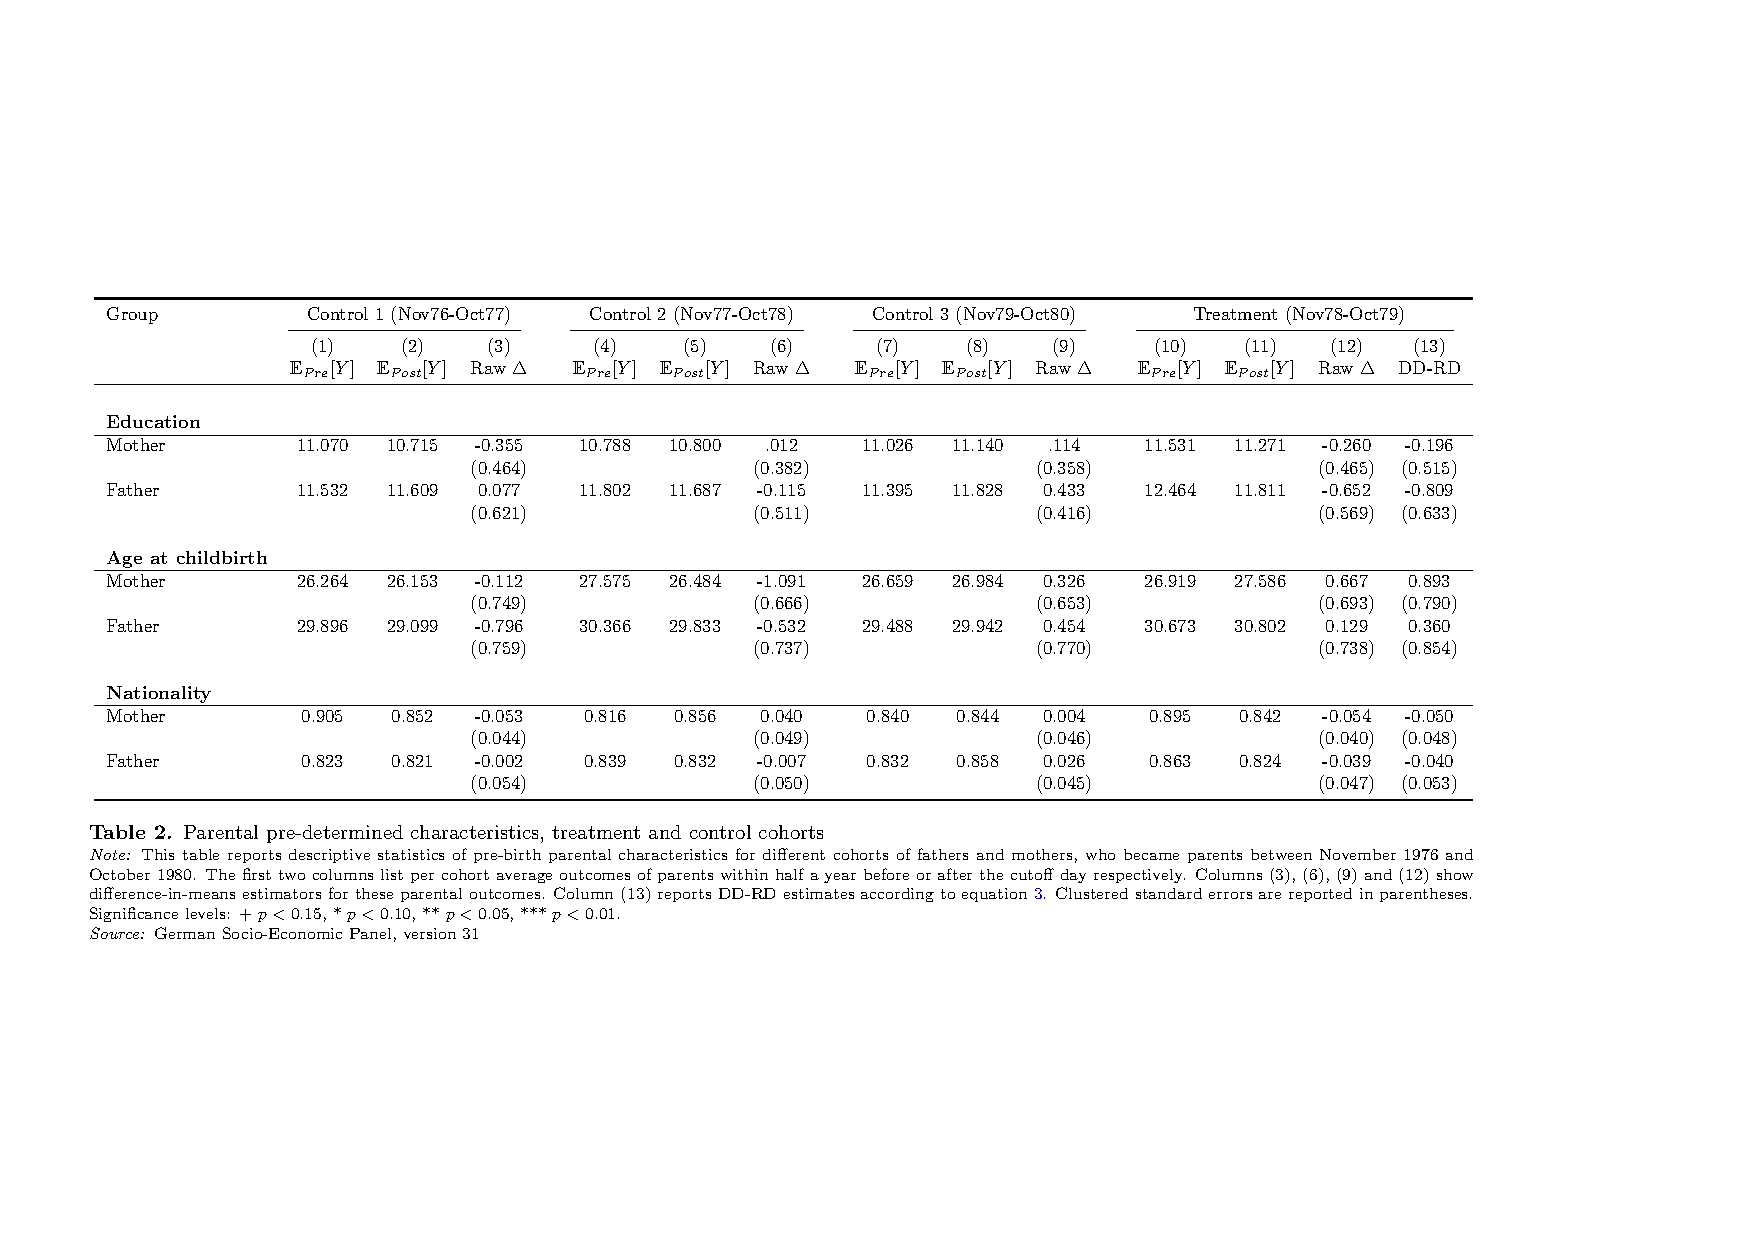
\includegraphics[width=\textwidth]{presentation/parents}};
%	\draw[red,ultra thick,rounded corners] (7.5,1) rectangle (10.5,5);
%	\end{tikzpicture}
%\end{figure}
%\end{frame}
%
%
%
%%------------------------------------------------------
%\begin{frame}
%\begin{figure}\label{HEALTHBEHAVIOR}
%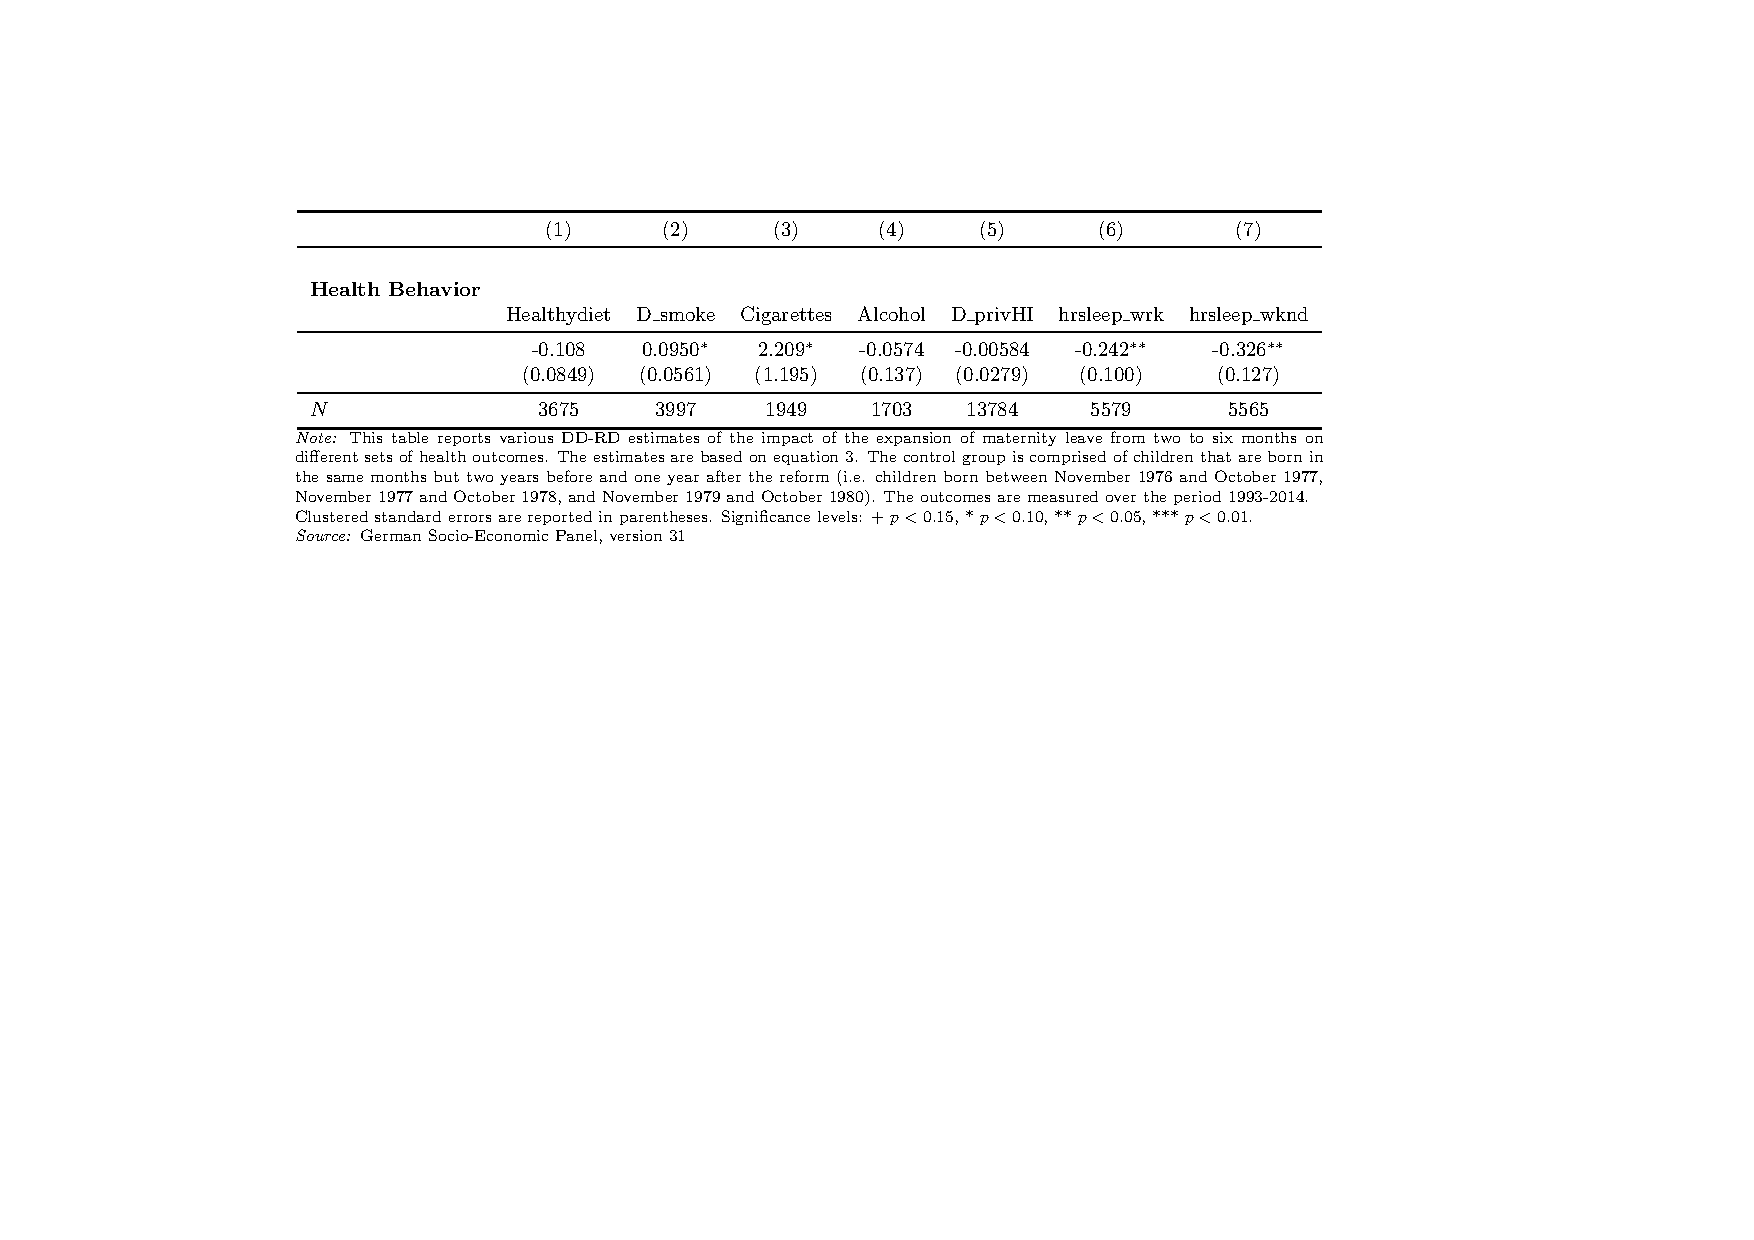
\includegraphics[width=\textwidth]{presentation/HealthBehavior}
%\end{figure}
%\hyperlink{BackMainResults}{\beamerbutton{Back to main results}}
%\end{frame}
%
%
%%------------------------------------------------------
%%MECHANISMS
%\begin{frame}{Mechanisms}
%\hyperlink{BACK_HETERO}{\beamerbutton{Back to Heterogeneity Analysis}}
%\begin{figure}\label{MECHANISMS}
%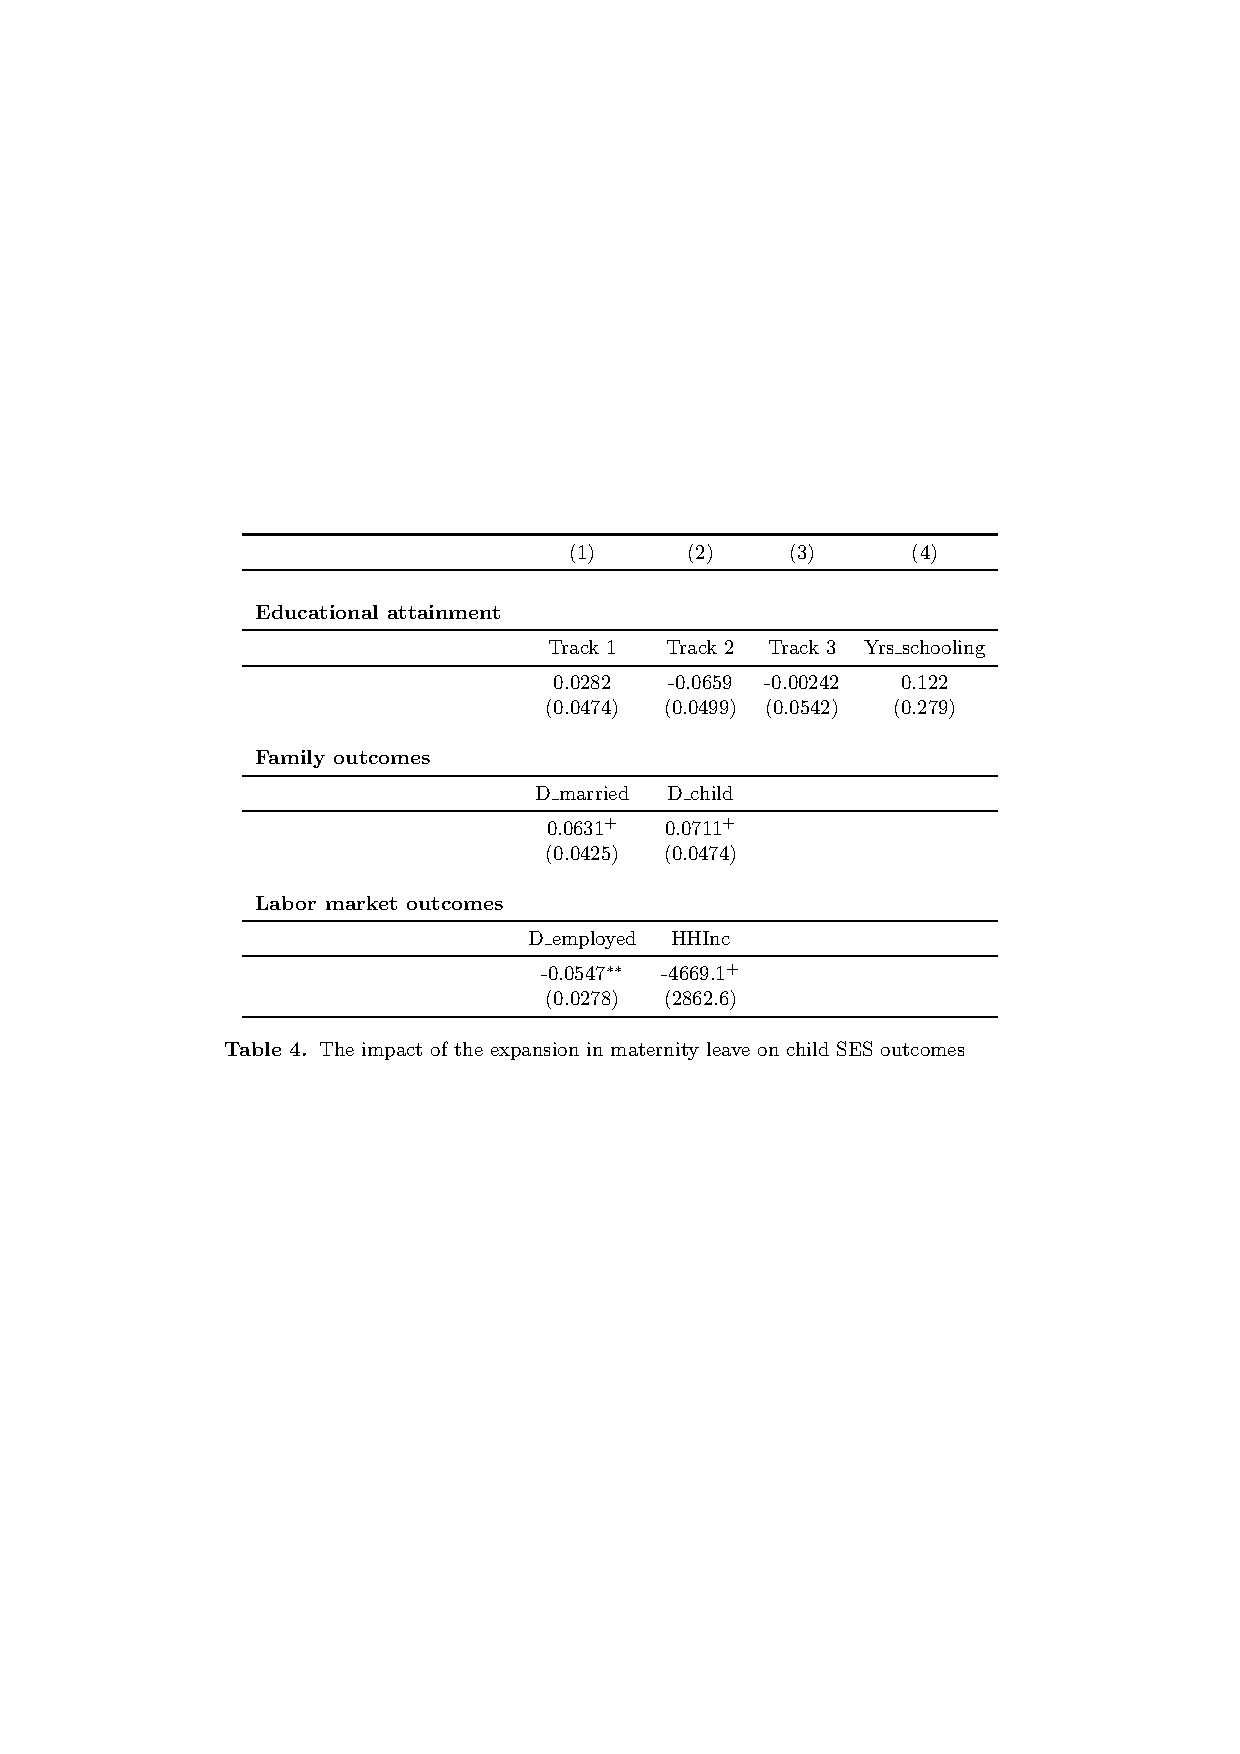
\includegraphics[width=0.75\textwidth]{presentation/Mechanisms_2}
%\end{figure}
%\begin{itemize}
%\item $\Rightarrow$ \mynum{1} and \mynum{3} are verified by D\&S (2012)
%\item \mynum{1} excluded, \mynum{3} possible explanation, \mynum{2} ambiguous effect
%\item Merely suggestive evidence
%\end{itemize}
%\end{frame}


\end{document}